%\documentclass[a4paper,12pt,twoside]{book}
\documentclass[12pt,times]{report}
\usepackage{mathptmx}%This package supersedes times and mathptm
\usepackage[a4paper,right=2.54cm,left=2.54cm,top=2.54cm,bottom=2.54cm]{geometry}

%%%%paquete para usar citas de diferentes formatos
%%%%%%%%%%%%%%%%%%%%%%%%%%%%%%%%%
%%add al indice
%\usepackage[nottoc,numbib]{tocbibind}
%\usepackage[authoryear,round]{natbib}
\usepackage[utf8]{inputenc}
\usepackage{csquotes}
\usepackage[spanish]{babel}
\usepackage[style=apa ,
%hyperref=auto,
%citestyle=authoryear,
natbib=true,
backend=biber]{biblatex}
\addbibresource{biblio/references.bib}
%\usepackage{biblatex}
%paquete para hiperlinks entre citas e imagenes
\usepackage{longtable}
\usepackage{ragged2e}
\usepackage{booktabs}
\usepackage{multirow}
%%%%%%%%%%%%%%%%%%%%%%%%%%%%%%%%%
\usepackage[colorlinks=true,
citecolor=blue,
urlcolor=cyan,
bookmarks=true,
linkcolor=blue,
pdftitle={Tesis-nombre-alumno},
pdfauthor={autor nombres}]{hyperref}

\usepackage{amssymb}
\usepackage{graphicx} % for improved inclusion of graphics
%\usepackage{wrapfig} % to include figure with text wrapping around it
\usepackage[margin=10pt,font=small,labelfont=bf]{caption} % for improved layout of figure captions with extra margin, smaller font than text
\usepackage{eucal}
\usepackage{float}

\usepackage[usenames, dvipsnames]{color}
\usepackage[perpage]{footmisc}
%\usepackage[round, sort]{natbib}
\usepackage{ifthen}
\usepackage{multicol} % for pages with multiple text columns, e.g. References
\setlength{\columnsep}{20pt} % space between columns; default 10pt quite narrow
\usepackage[nottoc]{tocbibind} % correct page numbers for bib in TOC, nottoc suppresses an entry for TOC itself
\usepackage{appendix}

%%%----Modificar encabezado y pie de pagina
%%%%%%%%%%%%%%%%%%%%%%%%%%%%%%%%%%%%%%%%%%%%%%%%%%%%%%%%%%%%%%%%%%%%%
\usepackage{fancyhdr} % for better header layout
\newcommand{\changefont}{%
	\fontsize{9pt}{1.5pt}\selectfont
}
\pagestyle{fancy}
\fancyhf{} %% delete default configuration of page
%%\setlength\headheight{15pt}
\fancyhead[L]{\changefont Trabajo de Tesis}
\fancyhead[R]{\changefont \leftmark}
%%\fancyfoot[L]{\leftmark}
\fancyfoot[R]{\thepage}

%%%%%%%%%%%%%%%%%%%%%%%%%%%%%5
%%%% Configuracion de los parrafos
%\usepackage{setspace}
%\onehalfspacing
%\linespread{1.25} 
\setlength{\parindent}{0.5in} %%sangria
\setlength{\parskip}{3mm}  %%espacio entre parrafos
\linespread{1.3} %This equals 1.5 linespacing in Word
%%%% nuevo parrafo
%%%%%%%%%%%%%%%%%%%%%%%%%%%%%5
%%%% Centrar valores de una tabla
\usepackage{array}
%%CENTRADO HORIZONTAL
\newcolumntype{P}[1]{>{\centering\arraybackslash}p{#1}}
%%CENTRADO VERTICAL
\newcolumntype{M}[1]{>{\centering\arraybackslash}m{#1}}

%%%%%%%%%%%%%%%%%%%%%%%%%%%%%5
%%%%Paquete para alinear texto
\usepackage{ragged2e}
\usepackage{multirow}
\usepackage{makecell}
\usepackage{rotating}
\usepackage{siunitx} % To align the numbers later on
\usepackage[table,xcdraw]{xcolor}
\usepackage{color, colortbl}
\definecolor{Gray}{gray}{0.9}
\definecolor{orange}{rgb}{1,0.647,0}
\definecolor{turq3}{rgb}{0.54, 0.81, 0.94}
\definecolor{turq}{rgb}{0.63, 0.79, 0.95}
\definecolor{bluejean}{rgb}{0.03, 0.27, 0.49}

%%%%%%%%%%%%%%%%%%%%%%%%%
\usepackage{xparse}
\usepackage{expl3}
%%%%funcion de reemplazar regex
\ExplSyntaxOn
\NewDocumentCommand{\replace}{mmm}
{
	\marian_replace:nnn {#1} {#2} {#3}
}

\tl_new:N \l_marian_input_text_tl
\tl_new:N \l_marian_search_tl
\tl_new:N \l_marian_replace_tl

\cs_new_protected:Npn \marian_replace:nnn #1 #2 #3
{
	\tl_set:Nn \l_marian_input_text_tl { #1 }
	\tl_set:Nn \l_marian_search_tl { #2 }
	\tl_set:Nn \l_marian_replace_tl { #3 }
	\regex_replace_all:nnN { \b\u{l_marian_search_tl}\b } { \u{l_marian_replace_tl} } \l_marian_input_text_tl
	\tl_use:N \l_marian_input_text_tl
}
\ExplSyntaxOff

%%%%%%%%%%%%%%%%%%%%%%%%%%%%%%%%%%%%%%
\usepackage{amsmath}
\numberwithin{equation}{chapter} %%enumerar ecuaciones
\renewcommand{\theequation}{Ecuación \thechapter.\arabic{equation}}   
\usepackage{mathtools, nccmath, cool}
%%%Configuraciones de biblatex

%%%hel
%%%%\citeauthor
\makeatletter

%%%%%%%%%%%%
\DeclareCiteCommand{\citeauthor}
{\boolfalse{citetracker}%
	\boolfalse{pagetracker}%
	\usebibmacro{prenote}}
{\ifciteindex
	{\indexnames{labelname}}
	{}%
	\printtext[bibhyperref]{\printnames{labelname}}}
{\multicitedelim}
{\usebibmacro{postnote}}


\DeclareCiteCommand{\citetitle}
{\boolfalse{citetracker}%
	\boolfalse{pagetracker}%
	\usebibmacro{prenote}}
{\ifciteindex
	{\indexfield{indextitle}}
	{}%
	\printtext[bibhyperref]{\printfield[citetitle]{labeltitle}}}
{\multicitedelim}
{\usebibmacro{postnote}}

\DeclareCiteCommand{\cite}
{\usebibmacro{prenote}}
{\usebibmacro{citeindex}%
	\printtext[bibhyperref]{\usebibmacro{cite}}}
{\multicitedelim}
{\usebibmacro{postnote}}

\DeclareCiteCommand*{\cite}
{\usebibmacro{prenote}}
{\usebibmacro{citeindex}%
	\printtext[bibhyperref]{\usebibmacro{citeyear}}}
{\multicitedelim}
{\usebibmacro{postnote}}

\DeclareCiteCommand{\parencite}[\mkbibparens]
{\usebibmacro{prenote}}
{\usebibmacro{citeindex}%
	\printtext[bibhyperref]{\usebibmacro{cite}}}
{\multicitedelim}
{\usebibmacro{postnote}}

\DeclareCiteCommand*{\parencite}[\mkbibparens]
{\usebibmacro{prenote}}
{\usebibmacro{citeindex}%
	\printtext[bibhyperref]{\usebibmacro{citeyear}}}
{\multicitedelim}
{\usebibmacro{postnote}}

\DeclareCiteCommand{\footcite}[\mkbibfootnote]
{\usebibmacro{prenote}}
{\usebibmacro{citeindex}%
	\printtext[bibhyperref]{ \usebibmacro{cite}}}
{\multicitedelim}
{\usebibmacro{postnote}}

\DeclareCiteCommand{\footcitetext}[\mkbibfootnotetext]
{\usebibmacro{prenote}}
{\usebibmacro{citeindex}%
	\printtext[bibhyperref]{\usebibmacro{cite}}}
{\multicitedelim}
{\usebibmacro{postnote}}

\DeclareCiteCommand{\textcite}
{\boolfalse{cbx:parens}}
{\usebibmacro{citeindex}%
	\printtext[bibhyperref]{\usebibmacro{textcite}}}
{\ifbool{cbx:parens}
	{\bibcloseparen\global\boolfalse{cbx:parens}}
	{}%
	\multicitedelim}
{\usebibmacro{textcite:postnote}}
\makeatother
\makeatletter
\let\abx@macro@citeOrig\abx@macro@cite
\renewbibmacro{cite}{%
	\bibhyperref{%
		\let\bibhyperref\relax\relax%
		\abx@macro@citeOrig%
	}%
}
\let\abx@macro@textciteOrig\abx@macro@textcite
\renewbibmacro{textcite}{%
	\bibhyperref{%
		\let\bibhyperref\relax\relax%
		\abx@macro@textciteOrig%
	}%
}%

\makeatother

%%%%%%%%%%%%%%%%%%%%%%%%%%%%%%%%%%%%%%%%%%%
\begin{document}

\begin{titlepage}

	\begin{center}
		%%%cargar imagen
	    
\includegraphics[width=0.45\textwidth]{images_repo/esanlogomin}
		\vspace*{2cm} \\
		UNIVERSIDAD ESAN \vspace*{1ex} \\
		FACULTAD DE INGENIERÍA \vspace*{1ex} \\
		INGENIERÍA DE TECNOLOGÍAS DE INFORMACIÓN Y SISTEMAS\vspace*{8ex} \\
		\textbf{Desarrollo de una aplicación móvil empleando Inteligencia Artificial generativa para el soporte integral a pacientes con cáncer de mama}
		\vspace*{8ex}\\	
		Trabajo de Tesis I 
		\vspace*{8ex} \\	
		Carlos Francisco Celi Garay \\
		Asesor: Marks Calderón		
		\vfill
		
		Lima, \today 
		
	\end{center}
\end{titlepage}
%%cambiar nombres de objetos para el indice y otros
\renewcommand{\listfigurename}{Índice de Figuras}
\renewcommand{\tablename}{Tabla}
\renewcommand{\listtablename}{Índice de Tablas}

\thispagestyle{plain}
\begin{center}
	\vspace*{1.5cm}
	{\Large \bfseries  Resumen}
\end{center}
\vspace{0.5cm}
Lorem ipsum dolor sit amet, consectetur adipiscing elit, sed do eiusmod tempor incididunt ut labore et dolore magna aliqua. Ac odio tempor orci dapibus ultrices in iaculis nunc sed. Vivamus arcu felis bibendum ut tristique et egestas quis ipsum. Odio morbi quis commodo odio aenean sed adipiscing diam donec. Donec ultrices tincidunt arcu non sodales neque sodales ut. Fusce ut placerat orci nulla pellentesque dignissim enim sit amet. Facilisi etiam dignissim diam quis enim lobortis. Sit amet justo donec enim diam vulputate ut pharetra. Gravida in fermentum et sollicitudin ac orci phasellus egestas. Ultricies tristique nulla aliquet enim tortor at auctor. Nullam vehicula ipsum a arcu cursus vitae congue mauris. Convallis posuere morbi leo urna molestie at elementum eu facilisis. Elit at imperdiet dui accumsan sit amet nulla. Amet consectetur adipiscing elit pellentesque habitant morbi tristique senectus et. Mauris in aliquam sem fringilla ut morbi. Ultricies integer quis auctor elit sed vulputate mi sit. Nulla pellentesque dignissim enim sit amet venenatis urna cursus eget. Ac feugiat sed lectus vestibulum mattis ullamcorper. Eu augue ut lectus arcu bibendum. Rhoncus dolor purus non enim praesent elementum. 

Nulla facilisi cras fermentum odio eu feugiat pretium. Massa massa ultricies mi quis hendrerit. Id leo in vitae turpis massa sed elementum. Quis vel eros donec ac odio tempor orci. Netus et malesuada fames ac turpis egestas integer eget aliquet. Velit ut tortor pretium viverra suspendisse potenti. Ut enim blandit volutpat maecenas. Nibh tellus molestie nunc non blandit. Mus mauris vitae ultricies leo integer malesuada nunc vel. Vel elit scelerisque mauris pellentesque pulvinar pellentesque habitant. Neque viverra justo nec ultrices dui sapien eget. Vitae aliquet nec ullamcorper sit. Dui id ornare arcu odio ut sem nulla pharetra diam. Et magnis dis parturient montes. Varius morbi enim nunc faucibus.
\newline

\textbf{Palabras claves: } uno, dos, tres, cuatro
\thispagestyle{plain}
\begin{center}
	\vspace*{1.5cm}
	{\Large \bfseries  Abstract}
\end{center}
\vspace{0.5cm}
Lorem ipsum dolor sit amet, consectetur adipiscing elit, sed do eiusmod tempor incididunt ut labore et dolore magna aliqua. Ac odio tempor orci dapibus ultrices in iaculis nunc sed. Vivamus arcu felis bibendum ut tristique et egestas quis ipsum. Odio morbi quis commodo odio aenean sed adipiscing diam donec. Donec ultrices tincidunt arcu non sodales neque sodales ut. Fusce ut placerat orci nulla pellentesque dignissim enim sit amet. Facilisi etiam dignissim diam quis enim lobortis. Sit amet justo donec enim diam vulputate ut pharetra. Gravida in fermentum et sollicitudin ac orci phasellus egestas. Ultricies tristique nulla aliquet enim tortor at auctor. Nullam vehicula ipsum a arcu cursus vitae congue mauris. Convallis posuere morbi leo urna molestie at elementum eu facilisis. Elit at imperdiet dui accumsan sit amet nulla. Amet consectetur adipiscing elit pellentesque habitant morbi tristique senectus et. Mauris in aliquam sem fringilla ut morbi. Ultricies integer quis auctor elit sed vulputate mi sit. Nulla pellentesque dignissim enim sit amet venenatis urna cursus eget. Ac feugiat sed lectus vestibulum mattis ullamcorper. Eu augue ut lectus arcu bibendum. Rhoncus dolor purus non enim praesent elementum. 

Nulla facilisi cras fermentum odio eu feugiat pretium. Massa massa ultricies mi quis hendrerit. Id leo in vitae turpis massa sed elementum. Quis vel eros donec ac odio tempor orci. Netus et malesuada fames ac turpis egestas integer eget aliquet. Velit ut tortor pretium viverra suspendisse potenti. Ut enim blandit volutpat maecenas. Nibh tellus molestie nunc non blandit. Mus mauris vitae ultricies leo integer malesuada nunc vel. Vel elit scelerisque mauris pellentesque pulvinar pellentesque habitant. Neque viverra justo nec ultrices dui sapien eget. Vitae aliquet nec ullamcorper sit. Dui id ornare arcu odio ut sem nulla pharetra diam. Et magnis dis parturient montes. Varius morbi enim nunc faucibus.
\newline

\textbf{Keywords: } uno, dos, tres, cuatro
\thispagestyle{plain}
\begin{center}
	\vspace*{1.5cm}
	{\Large Para mi X, Y,X}
\end{center}


\thispagestyle{plain}
\begin{center}
	\vspace*{1.5cm}
	{\Large \bfseries  Agradecimientos}
\end{center}
\vspace{0.5cm}
Lorem ipsum dolor sit amet, consectetur adipiscing elit, sed do eiusmod tempor incididunt ut labore et dolore magna aliqua. Ac odio tempor orci dapibus ultrices in iaculis nunc sed. Vivamus arcu felis bibendum ut tristique et egestas quis ipsum. Odio morbi quis commodo odio aenean sed adipiscing diam donec. Donec ultrices tincidunt arcu non sodales neque sodales ut. Fusce ut placerat orci nulla pellentesque dignissim enim sit amet. Facilisi etiam dignissim diam quis enim lobortis. Sit amet justo donec enim diam vulputate ut pharetra. Gravida in fermentum et sollicitudin ac orci phasellus egestas. Ultricies tristique nulla aliquet enim tortor at auctor. Nullam vehicula ipsum a arcu cursus vitae congue mauris. Convallis posuere morbi leo urna molestie at elementum eu facilisis. Elit at imperdiet dui accumsan sit amet nulla. Amet consectetur adipiscing elit pellentesque habitant morbi tristique senectus et. Mauris in aliquam sem fringilla ut morbi. Ultricies integer quis auctor elit sed vulputate mi sit. Nulla pellentesque dignissim enim sit amet venenatis urna cursus eget. Ac feugiat sed lectus vestibulum mattis ullamcorper. Eu augue ut lectus arcu bibendum. Rhoncus dolor purus non enim praesent elementum. 

Nulla facilisi cras fermentum odio eu feugiat pretium. Massa massa ultricies mi quis hendrerit. Id leo in vitae turpis massa sed elementum. Quis vel eros donec ac odio tempor orci. Netus et malesuada fames ac turpis egestas integer eget aliquet. Velit ut tortor pretium viverra suspendisse potenti. Ut enim blandit volutpat maecenas. Nibh tellus molestie nunc non blandit. Mus mauris vitae ultricies leo integer malesuada nunc vel. Vel elit scelerisque mauris pellentesque pulvinar pellentesque habitant. Neque viverra justo nec ultrices dui sapien eget. Vitae aliquet nec ullamcorper sit. Dui id ornare arcu odio ut sem nulla pharetra diam. Et magnis dis parturient montes. Varius morbi enim nunc faucibus.
\newline



% outline
\tableofcontents            % print the table of contents

%: ----------------------- contents ------------------------

\setcounter{secnumdepth}{3} % organisational level that receives a numbers
\setcounter{tocdepth}{3}    % print table of contents for level 3

% levels are: 0 - chapter, 1 - section, 2 - subsection, 3 - subsection


%: ----------------------- list of figures/tables ------------------------

\listoffigures	% print list of figures

\listoftables  % print list of tables



\chapter{PLANTEAMIENTO DEL PROBLEMA}
En el presente capítulo se mostrará el cáncer como una enfermedad mortal presente en todo el mundo. (Se mejorará cuando se concluya el capítulo).
\section{Descripción de la Realidad Problemática}

El cáncer es una de las enfermedades más mortales que puede manifestarse en cualquier etapa de la vida de una persona, convirtiéndose en un problema de salud pública a nivel mundial. Según datos de la Organización Mundial de la Salud (OMS) y la Sociedad Americana de Cáncer, el riesgo global de desarrollar cáncer se estima en 20.2\% para individuos de 0 a 74 años, y cerca de 10 millones de defunciones fueron atribuidas a esta enfermedad en 2020. Se ha determinado que uno de cada dos hombres y una de cada tres mujeres será diagnosticado con cáncer en algún momento de su vida. Además, cerca de 400 000 niños contraen cáncer cada año.

A nivel global, los tres tipos de cáncer más comunes fueron el de mama (2.26 millones de casos), pulmón (2.21 millones de casos) y colorrectal (1.93 millones de casos). Por otro lado, los más mortales fueron el de pulmón (1.8 millones de defunciones), colorrectal (916 000 defunciones) y hepático (830 000 defunciones). La carga de la enfermedad asociada al cáncer es muy alta, siendo responsable de 2668.475 millones de años de vida ajustados por discapacidad, lo que lo convierte en una de las enfermedades con mayor impacto a nivel mundial.

En América Latina y el Caribe, la situación es igualmente crítica. De acuerdo con los datos de GLOBOCAN 2022, se reportaron aproximadamente 1.55 millones de nuevos casos de cáncer en la región durante ese año, con 700 mil muertes, lo que equivale a una tasa de incidencia de 186.0 por cada 100 mil habitantes y una tasa de mortalidad de 233.1 por cada 100 mil habitantes. Se estima que la carga de la enfermedad continuará aumentando, y para el año 2040 la incidencia del cáncer en la región podría incrementarse en un 69\%. A pesar de los avances en la lucha contra el cáncer en América Latina y el Caribe, persisten problemas críticos como los sistemas de salud fragmentados, la inequidad en el acceso a servicios médicos, la falta de registros adecuados y el acceso limitado a datos. Todo esto hace urgente mejorar el control del cáncer en la región.

En la Figura \ref{1:fig} y Figura \ref{2:fig} se observa la distribución del cáncer a nivel global, tanto en incidencia como en mortalidad, recolectados por GLOBOCAN 2022.%\medskip

\begin{figure}[ht]
    \centering
    % Primera figura
    \begin{minipage}[b]{0.48\textwidth}
        \centering
        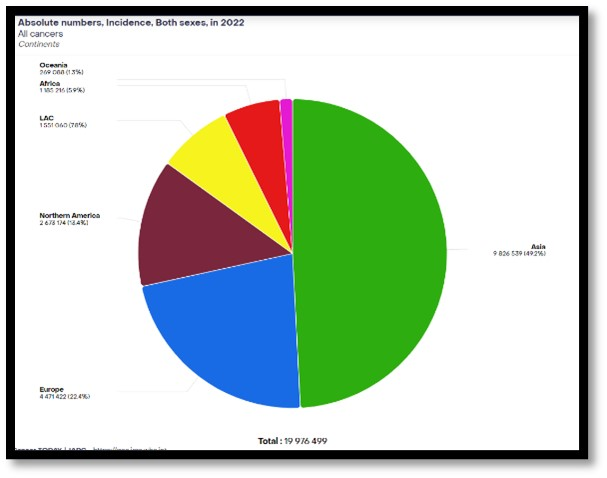
\includegraphics[width=\textwidth]{1/figures/Incidencias.jpg}
        \caption{Números absolutos, Incidencia, Ambos sexos, en 2022 (Todos los cánceres, todos los continentes). Fuente:\cite{iarc}}
        \label{1:fig}
    \end{minipage}
    \hfill
    % Segunda figura
    \begin{minipage}[b]{0.48\textwidth}
        \centering
        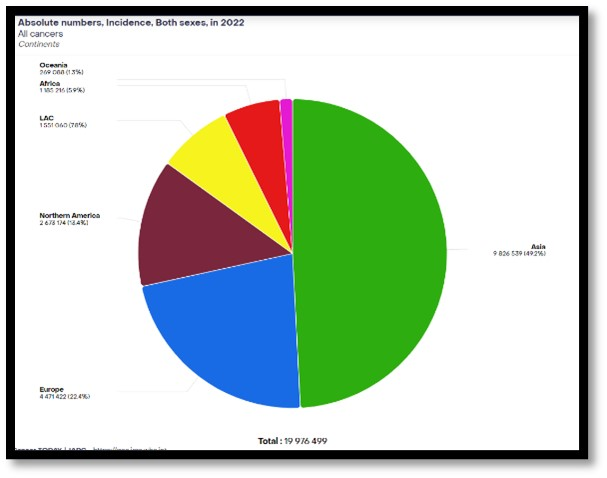
\includegraphics[width=\textwidth]{1/figures/Incidencias.jpg}
        \caption{Números absolutos, Mortalidad, Ambos sexos, en 2022 (Todos los cánceres, todos los continentes). Fuente:\cite{iarc}}
        \label{2:fig}
    \end{minipage}
\end{figure}

Considerando el impacto global del cáncer, es importante enfocarnos en el contexto nacional. En Perú, esta enfermedad representa una de las principales causas de mortalidad y ha sido declarada una prioridad por el Ministerio de Salud (Minsa) y el Seguro Social de Salud (EsSalud). La Agencia Internacional para la Investigación en Cáncer (IARC) estimó para 2020 un total de 69 869 nuevos casos de cáncer en Perú y 34 976 defunciones por cáncer.

Mediante la información recolectada por el Centro Nacional de Epidemiología, Prevención y Control de Enfermedades, podemos observar la tendencia y distribución de casos registrados de pacientes con cáncer en las Figuras N°\ref{3:fig} y N°\ref{4:fig}

\begin{figure}[ht]
	\centering
	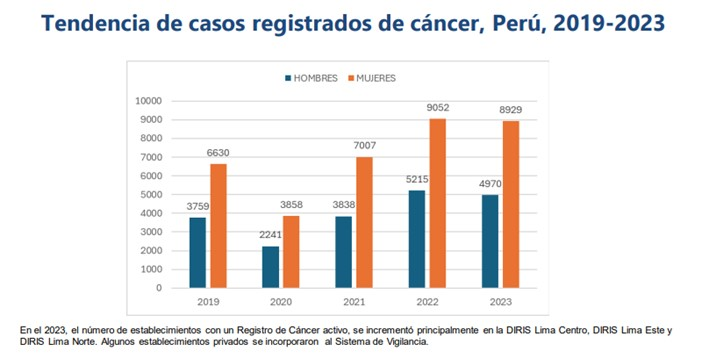
\includegraphics[width=1.1\textwidth]{1/figures/Tendencia.jpg}
	\caption{Tendencia de casos registrados de cáncer, Perú, 2019-2023. Fuente: \cite{cdc2023cancer}}
	\label{3:fig}
\end{figure}

\begin{figure}[h!]
	\centering
	\includegraphics[width=1.1\textwidth]{1/figures/Distribución.jpg}
	\caption{Distribución de casos registrados de cáncer por edad y sexo, Perú, 2023. Fuente: \cite{cdc2023cancer}}
	\label{4:fig}
\end{figure}

Se obtuvo que una proporción significativa de casos le pertenece al cáncer de mama. Este tipo de cáncer afecta a miles de mujeres cada año, y su diagnóstico en etapas avanzadas aumenta la complejidad del tratamiento y reduce las posibilidades de supervivencia.
El cáncer de mama es el tipo de cáncer más frecuente en mujeres peruanas, y sus efectos son devastadores tanto física como emocionalmente. Esta enfermedad no solo amenaza la vida de las pacientes, sino que también conlleva profundas repercusiones en su bienestar emocional, social y económico. Las mujeres con cáncer de mama pueden experimentar síntomas como la aparición de un bulto en el seno, cambios en la forma o tamaño del seno, secreción del pezón, y dolor en las mamas. Sin embargo, muchas veces, los síntomas no son evidentes en las primeras etapas, lo que dificulta la detección temprana y aumenta el riesgo de que la enfermedad avance a estadios más peligrosos.
Cuando el cáncer de mama se diagnostica en etapas avanzadas, las consecuencias son mucho más graves. El tratamiento suele ser más invasivo y costoso, e implica quimioterapia, radioterapia o cirugías complejas como la mastectomía, que afecta significativamente la imagen corporal de la mujer. Además del impacto físico, las pacientes pueden sufrir una fuerte carga emocional, ya que el tratamiento conlleva efectos secundarios como pérdida de cabello, fatiga extrema, náuseas y un estado de vulnerabilidad emocional que puede llevar a la ansiedad y la depresión. La enfermedad no solo afecta a la paciente, sino también a su entorno familiar, social y laboral, generando una carga financiera y emocional considerable.
El cáncer de mama no tratado a tiempo puede diseminarse a otras partes del cuerpo, como los huesos, los pulmones o el hígado, lo que se conoce como metástasis, lo que disminuye drásticamente las probabilidades de supervivencia. En Perú, la situación es especialmente preocupante debido a la alta tasa de diagnósticos en etapas avanzadas. La mayoría de las mujeres que desarrollan cáncer de mama provienen de áreas rurales o poblaciones vulnerables, donde el acceso a servicios médicos es limitado, y la falta de información sobre la autoexploración y los chequeos médicos regulares es alarmante. Esta distribución se puede observar en la Figura N°\ref{5:fig}.
\begin{figure}[ht]
	\centering
	\includegraphics[width=1.1\textwidth]{1/figures/Estadificación.jpg}
	\caption{Estadificación del cáncer en los casos registrados, Perú, 2023. Fuente: \cite{cdc2023cancer}}
	\label{5:fig}
\end{figure}
\vspace{0.5 cm}

Donde en el país los costos de tratamiento son altos pueden rondar entre los 200 000 soles a los 450 000 soles como mínimo (Aproximadamente pueden variar) que pueden incluir gastos en consultas médicas, exámenes de laboratorio, exámenes por imágenes, radioterapias, quimioterapias entre otros. Podemos darnos cuenta de esto mirando el tarifario por ejemplo del instituto nacional de enfermedades de neoplásicas en la figura N°\ref{6:fig}, solo para quimioterapia rondan entre los 37 soles a 595 soles teniendo en cuenta la eficacia y la rapidez de la atención, esto solo es la administración ya que los medicamentos administrados es otro precio a parte que incrementan el precio de la sesión.

\begin{figure}[ht]
	\centering
	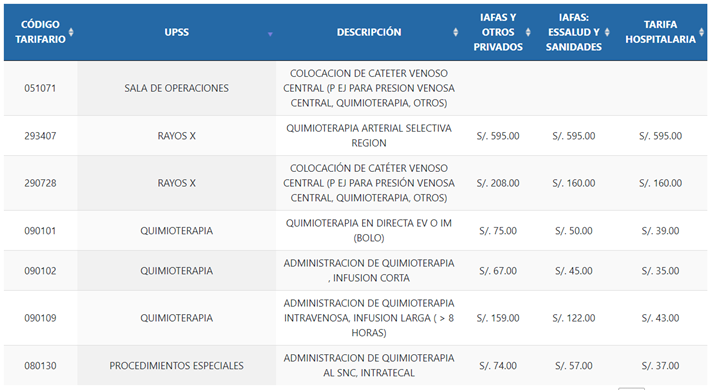
\includegraphics[width=1.1\textwidth]{1/figures/Tarifario.png}
	\caption{Tarifario- Quimioterapia. Fuente: \cite{inenTarifario}}
	\label{6:fig}
\end{figure}
\vspace{0.5 cm}

Sabiendo esto para un peruano seria vital tener un seguro oncológico, por el lado privado tendríamos a Oncosalud como ejemplo que brindan planes de cobertura con tarifas mensuales que incluyen gastos en medicamentos, tratamientos, citas médicas, entre otros, cabe resaltar que al optar por esta opción se debe tener en cuenta cuanto cubre y que cosas no.

Por el lado publico es un poco más complicado, teniendo que el Perú es un país donde desborda el trabajo informal y población de escasos recursos tanto en zona urbana y rural donde una gran cantidad de la población no con cuenta con seguro integral de Salud (SIS) o seguro social de salud (EsSalud), se puede apreciar esto en la figura N°\ref{7:fig}.

\begin{figure}[ht]
	\centering
	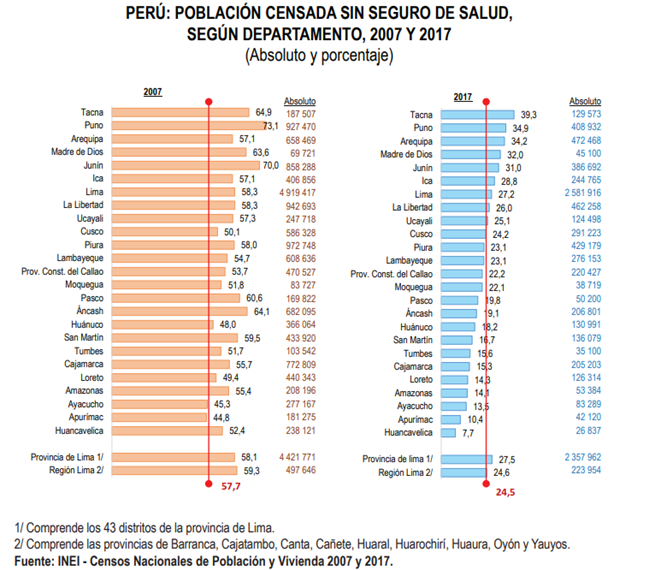
\includegraphics[width=1.1\textwidth]{1/figures/SINSEGURO.png}
	\caption{Población censada sin seguro de salud, según departamento, 2007 y 2017. Fuente: \cite{inei2018poblacion}}
	\label{7:fig}
\end{figure}

Sin embargo, en la población hay una gran tasa de desinformación y poco interés sobre el cáncer. Según la encuesta de Oncosalud junto a Ipsos Perú, se determinó que hombres y mujeres de 18 a 65 años no se sienten protegidos contra el cáncer y solo un 34\% de personas se sienten listas para enfrentar esta enfermedad a nivel de acceso al tratamiento y económico. Se obtuvo también que más de la mitad de los peruanos nunca se ha realizado un chequeo oncológico esta alta cifra se debe a la falta de información y al miedo de enfrentar la enfermedad.
Considerando todos estos factores, es importante señalar que el sistema de salud pública en Perú enfrenta deficiencias significativas. A pesar de que existen seguros públicos, no son suficientes para cubrir las necesidades de los pacientes debido a las largas colas, la escasez de medicamentos, la mala infraestructura, entre otros problemas que impiden una atención adecuada para enfrentar esta enfermedad. Además, una gran parte de la población vive en condiciones de pobreza o en zonas rurales donde el acceso a la información y a los servicios médicos es extremadamente limitado, lo que agrava la carga tanto para los pacientes como para sus familias. Esto se traduce en la acumulación de informes médicos, medicamentos, efectos secundarios, y otros factores que afectan gravemente la salud mental, un componente esencial para el bienestar general.
Si bien la medicina a avanzado junto con la tecnología haciendo un poco más fácil el tratamiento y la detección de esta enfermedad, se centra en eso, en decirle al paciente que tiene la enfermedad y ya. Y si tienes el dinero suficiente puedes tener todos los recursos para poder luchar contra la enfermedad, pero por el otro lado si no lo tienes estas condenado a morir.
Dada la magnitud de este desafío, es imperativo buscar soluciones innovadoras que puedan mitigar estos impactos adversos, especialmente en lugares donde el acceso a la información y a los servicios médicos es limitado. Aquí es donde las aplicaciones móviles entran en juego como un recurso vital. Según Okolo et al. (2024), que revisa el rol de las aplicaciones móviles en mejorar el compromiso del paciente y los resultados de salud, estas herramientas tecnológicas ofrecen un medio efectivo para gestionar la enfermedad de manera más eficiente. Las aplicaciones móviles no solo pueden facilitar el monitoreo constante de los signos vitales de los pacientes, sino que también permiten un acceso más fácil a información vital, mejorando la comunicación entre pacientes y proveedores de salud, y ofreciendo educación sobre la enfermedad que puede ser crucial para la detección temprana y la gestión efectiva del cáncer.
Aprovechando la tecnología móvil, los pacientes pueden superar las barreras geográficas y económicas que a menudo complican el acceso a tratamientos adecuados. Las aplicaciones pueden guiar a los usuarios en el proceso de autoexaminación, recordarles sus citas médicas y ciclos de medicación, y proporcionar información valiosa sobre los efectos secundarios y el manejo de la enfermedad. Esta interacción continua y accesible ayuda a reducir las colas en los hospitales, minimiza la escasez de medicamentos al permitir un mejor planeamiento y seguimiento, y puede mejorar significativamente la infraestructura de salud al reducir la carga sobre los recursos físicos.
En resumen, frente a un panorama tan desafiante como el del cáncer en Perú y en el mundo, es esencial integrar y aprovechar las tecnologías móviles para mejorar la atención del cáncer. No solo se trata de diagnosticar y tratar, sino de ofrecer una plataforma continua de apoyo y manejo que pueda hacer una diferencia significativa en la vida de los pacientes y sus familias, mejorando su calidad de vida y posiblemente sus tasas de supervivencia. Las aplicaciones móviles ofrecen una promesa tangible en esta lucha, demostrando ser no solo una necesidad sino una solución viable en el manejo moderno del cáncer.





\section{Formulación del Problema}

Habiendo presentado anteriormente el problema del cáncer tanto en el Perú y resto del mundo, podemos decir que la tecnología puede ayudar a los pacientes de cáncer, utilizando como herramienta algo que todos tienen un teléfono móvil, se presenta a continuación la formulación del problema central y los problemas específicos.

\subsection{Problema General}

\begin{itemize}
	\item \textit{PG} : ¿De qué manera una aplicación móvil mediante el uso de inteligencia artificial generativa puede contribuir al control, monitoreo integral y educación de los pacientes con cáncer de mama?
 
\end{itemize}

 \subsection{Problemas específicos}
 \begin{itemize}
         \item \textit{PE 1} : ¿Qué base de datos se deben usar para entrenar el modelo de inteligencia artificial para ofrecer respuestas optimas?
         \item \textit{PE 2} : ¿De qué manera una aplicación móvil puede proporcionar soporte emocional a los pacientes oncológicos?
         \item \textit{PE 3} : ¿Qué funcionalidades de una aplicación móvil son esenciales para el monitoreo de signos vitales en pacientes con cáncer?
          \item \textit{PE 4} : ¿Cómo puede una aplicación móvil proporcionar información personalizada y actualizada sobre el cáncer de mama utilizando IA generativa?
          \item \textit{PE 5} : ¿Qué modelo de IA generativa se va a implementar para que las funciones de la aplicación móvil funcionen correctamente?
          

\end{itemize}

\section{Objetivos de la Investigación}
A continuación, se presentarán el objetivo central y específicos de esta investigación.

\subsection{Objetivo General}
\begin{itemize}
	\item \textit{OG} : Desarrollar una aplicación móvil basada en Inteligencia Artificial generativa para el monitoreo integral y el control de pacientes con cáncer, que mejore la adherencia al tratamiento, el seguimiento de signos vitales, el soporte emocional y conocimiento sobre la enfermedad.
 
\end{itemize}

 \subsection{Objetivos específicos}
 \begin{itemize}
         \item \textit{OE 1} : Identificar las bases de datos especializadas que se pueden integrar para entrenar el modelo de IA generativa de la aplicación móvil.
         \item \textit{OE 2} : Implementar un sistema de IA generativa que proporcione soporte emocional personalizado en función del estado anímico del paciente.
         \item \textit{OE 3} : Desarrollar e integrar un sistema de monitoreo de signos vitales en tiempo real que notifique a los pacientes sobre anomalías.
         \item \textit{OE 4} : Desarrollar una funcionalidad que permita a los pacientes recibir información personalizada y actualizada sobre su condición.
         \item \textit{OE 5} : Seleccionar y optimizar el modelo de IA generativa más adecuado para integrar todas las funciones de la aplicación móvil de manera eficiente.
\end{itemize}
\section{Hipótesis General}
En este presente trabajo de investigación, se pretende comprobar que la utilización de una aplicación móvil mejorar en el soporte integral de un paciente con cáncer de mama. La hipótesis general del presente proyecto de investigación es la siguiente.
\subsection{Hipótesis general }
\begin{itemize}
	\item \textit{HG} : El desarrollo de una aplicación móvil que emplea Inteligencia Artificial generativa mejorará significativamente el monitoreo integral, el control y la educación de pacientes con cáncer de mama.
 
\end{itemize}

\subsection{Hipótesis específicos}
 \begin{itemize}
         \item \textit{HE 1} : El desarrollo de una aplicación móvil que emplea Inteligencia Artificial generativa mejorará significativamente el soporte integral y la educación de pacientes con cáncer de mama.
         \item \textit{HE 2} : La implementación de un sistema de soporte emocional automatizado mejorará el bienestar emocional de los pacientes, reduciendo su ansiedad y mejorando su calidad de vida.
         \item \textit{HE 3} : La integración de un sistema de monitoreo de signos vitales basado en IA reducirá las complicaciones relacionadas con la falta de detección temprana de problemas.
         \item \textit{HE 4} : La implementación de un sistema que proporcione información personalizada mejorará el conocimiento del paciente sobre su enfermedad y su tratamiento.
         \item \textit{HE 5} : La implementación de un modelo de IA generativa optimizado permitirá que todas las funciones de la aplicación móvil (soporte emocional, monitoreo de signos vitales, información personalizada) funcionen de manera eficiente y precisa.
         

\end{itemize}

\section{Justificación de la Investigación}
A continuación, se presentarán la justificación teórica, práctica y metodológica para la elaboración de este proyecto.
\subsection{Justificación Teórica}
El cáncer de mama representa una de las principales causas de mortalidad a nivel mundial, lo que subraya la urgente necesidad de mejorar el soporte integral a los pacientes, abarcando tanto el monitoreo de su salud como el apoyo emocional y psicológico durante su tratamiento \parencite{pascucci2021}. La literatura científica reciente ha puesto de manifiesto la importancia crítica de desarrollar soluciones tecnológicas innovadoras que permitan a los pacientes acceder de manera rápida y efectiva a información personalizada sobre su condición, así como facilitar un monitoreo continuo y preciso de su salud \parencite{okolo2024}.

Los avances significativos en el campo de la inteligencia artificial, particularmente en el área de la IA generativa, ofrecen oportunidades sin precedentes para crear herramientas de atención médica altamente personalizadas. Esto se evidencia en la aplicación exitosa de modelos de lenguaje natural y algoritmos sofisticados de procesamiento de datos médicos en diversas áreas de la oncología \parencite{ce2024}. Estos modelos avanzados no solo permiten ofrecer recomendaciones y respuestas en tiempo real, sino que también tienen el potencial de asistir en la detección temprana de complicaciones relacionadas con el cáncer de mama, como cambios sutiles en los signos vitales o la aparición de lesiones cutáneas que podrían pasar desapercibidas \parencite{naeem2022}.

En paralelo, la aplicación de tecnologías móviles en el ámbito de la salud ha demostrado ser un medio excepcionalmente eficaz para mejorar la adherencia de los pacientes a sus tratamientos y promover la autogestión efectiva de sus condiciones crónicas \parencite{masciantonio2017}. Las aplicaciones móviles de salud han sido utilizadas con éxito para monitorear parámetros críticos, mejorar la comunicación bidireccional entre pacientes y médicos, y ofrecer un apoyo emocional continuo, aspectos que son particularmente cruciales para pacientes oncológicos que experimentan altos niveles de estrés y ansiedad durante su tratamiento \parencite{leung2022}.

En este contexto, el desarrollo de una aplicación móvil que integre de manera innovadora la IA generativa con el monitoreo exhaustivo de la salud busca atender de manera holística las múltiples y complejas necesidades de los pacientes con cáncer de mama. Al incorporar funcionalidades avanzadas como la detección precisa de signos vitales, un soporte emocional adaptativo, y la posibilidad de acceder a recomendaciones personalizadas sobre nutrición y manejo del tratamiento, la aplicación no solo empodera a los pacientes, sino que también tiene el potencial de mejorar significativamente sus resultados de salud a largo plazo \parencite{beltran2023}.

Además, es importante destacar el potencial de esta tecnología para abordar las disparidades en el acceso a la atención médica, especialmente en regiones con recursos limitados o en áreas rurales donde el acceso a especialistas oncológicos puede ser restringido \parencite{smith2023}. La aplicación móvil propuesta podría servir como un puente vital, proporcionando información crucial y monitoreo continuo a pacientes que de otra manera podrían tener un acceso limitado a estos recursos.

En conclusión, esta tesis se justifica en la creciente y apremiante necesidad de ofrecer a los pacientes con cáncer de mama un sistema integral y tecnológicamente avanzado de soporte a través de la convergencia de tecnologías innovadoras como la IA generativa y las aplicaciones móviles de salud. La implementación de una aplicación móvil de estas características permite abordar de manera efectiva los múltiples desafíos que enfrentan los pacientes, mejorando significativamente la accesibilidad a información personalizada, asegurando la continuidad en el monitoreo de su estado de salud, y elevando la calidad del soporte emocional que reciben. Estos elementos son fundamentales para el manejo efectivo y humanizado del cáncer de mama en la era digital.


\subsection{Justificación Práctica}
El cáncer de mama no solo es una de las principales causas de mortalidad en el mundo, sino que también representa un desafío significativo en el monitoreo continuo y en el soporte emocional para los pacientes. Las barreras de acceso a atención especializada y las limitaciones en el seguimiento personalizado de los tratamientos son problemas comunes en los sistemas de salud, especialmente en países de bajos y medianos ingresos \parencite{pascucci2021}. En este contexto, el desarrollo de una aplicación móvil que integre múltiples funcionalidades para el soporte de pacientes con cáncer de mama ofrece una solución práctica y viable.

El uso de aplicaciones móviles en el sector salud ha demostrado ser una herramienta eficiente para la autogestión de enfermedades crónicas, facilitando la adherencia a tratamientos y mejorando la comunicación entre pacientes y médicos \parencite{okolo2024}. La incorporación de IA generativa en esta aplicación permitirá generar respuestas personalizadas en tiempo real y ofrecer recomendaciones basadas en el análisis continuo de los datos de salud de los pacientes, como sus signos vitales y reportes de síntomas \parencite{ce2024}.

En la práctica, esta aplicación se presenta como una herramienta accesible para pacientes con cáncer de mama que enfrentan barreras geográficas o económicas para acceder a atención médica regular \parencite{leung2022}. Mediante el uso de smartphones, la aplicación permitirá el monitoreo remoto y la detección temprana de complicaciones, tales como cambios en los signos vitales o la aparición de nuevas lesiones en la piel. Esto reducirá la necesidad de visitas presenciales y permitirá una intervención médica más oportuna y eficiente \parencite{masciantonio2017}. Además, se ofrecerán recomendaciones personalizadas sobre nutrición, soporte emocional y manejo de tratamientos, lo que aumentará el compromiso de los pacientes y mejorará sus resultados de salud a largo plazo \parencite{beltran2023}.

El enfoque práctico de esta tesis radica en ofrecer una solución tecnológica integrada que no solo ayuda a los pacientes, sino que también reduce la carga en los sistemas de salud al permitir un seguimiento más eficiente y continuo sin depender completamente de consultas médicas presenciales \parencite{pascucci2021}. Los médicos podrán tomar decisiones más informadas y rápidas gracias a la disponibilidad de datos en tiempo real, mejorando la calidad del tratamiento y el bienestar del paciente. La aplicación es de fácil implementación y escalable, lo que significa que podría adaptarse para otros tipos de cáncer o enfermedades crónicas, generando un impacto positivo en la atención de la salud a nivel global.

En resumen, el desarrollo de esta aplicación móvil con IA generativa responde a una necesidad práctica urgente en el manejo integral de pacientes con cáncer de mama, facilitando el acceso a información personalizada, el monitoreo continuo de su salud y el soporte emocional. Esto mejorará su calidad de vida, reducirá las barreras al tratamiento y optimizará el uso de recursos en los sistemas de salud.

\subsection{Metodológica}. 
La investigación propone el desarrollo de una aplicación móvil con inteligencia artificial (IA) generativa para el soporte integral de pacientes con cáncer de mama. Para alcanzar este objetivo, la metodología se basa en la integración de herramientas tecnológicas avanzadas, tales como el aprendizaje automático (Machine Learning), el procesamiento de lenguaje natural (Natural Language Processing, NLP), entre otros. Estos elementos se combinan para ofrecer una solución innovadora que permita un monitoreo continuo y en tiempo real de los pacientes, así como recomendaciones personalizadas sobre su tratamiento y estado de salud.

La implementación de esta metodología tiene como principal aporte la creación de un sistema que puede interpretar y analizar grandes cantidades de datos clínicos relacionados con esta enfermedad. Este sistema permitirá detectar patrones en los signos vitales y otros indicadores de salud que podrían no ser percibidos por el paciente o el médico en una consulta regular. Al utilizar redes neuronales y modelos de IA generativa, el sistema podrá ofrecer recomendaciones adaptativas en tiempo real, basadas en el comportamiento y las necesidades específicas de cada paciente \parencite{ce2024}.

El instrumento principal de investigación es la aplicación móvil, que estará equipada con varias funcionalidades clave: el monitoreo de signos vitales mediante dispositivos móviles, interpretación de informes, un módulo de soporte emocional, calendarios personalizados y una plataforma para consultas automatizadas. Los datos capturados por los dispositivos móviles serán analizados mediante algoritmos de IA generativa entrenados en bases de datos clínicas, lo que permitirá la detección temprana de posibles complicaciones oncológicas \parencite{masciantonio2017}. Adicionalmente, se emplearán técnicas de procesamiento de imágenes para la detección de lesiones cutáneas, un aspecto crítico en la monitorización del cáncer de mama \parencite{leung2022}.

Para validar la eficacia de los algoritmos empleados, se llevará a cabo un proceso de validación comparativa utilizando bases de datos clínicas reales, las cuales contienen información de pacientes con cáncer de mama. Este método de validación, basado en la comparación con datos clínicos reales, permitirá evaluar la precisión del sistema en la detección y monitoreo de síntomas, así como en la generación de recomendaciones personalizadas. Además, se realizarán pruebas piloto con grupos de pacientes, con el fin de medir el impacto de la aplicación en la calidad de vida de los usuarios y en su adherencia al tratamiento \parencite{beltran2023}.

Desde una perspectiva metodológica, el uso de IA generativa en esta investigación representa un avance significativo en el ámbito de la salud digital. La aplicación de esta tecnología en el monitoreo continuo de la salud permitirá no solo mejorar la calidad de vida de los pacientes con cáncer de mama, sino que también contribuirá al desarrollo de nuevas metodologías en el campo de la telemedicina. Además, la capacidad de la aplicación para ser escalable y replicable en otras enfermedades crónicas refuerza su valor metodológico, al ofrecer una solución que puede ser adaptada a diferentes contextos clínicos.

\section{Delimitación del Estudio}
En este apartado se presentarán la delimitación espacial, temporal y conceptual del presente trabajo de investigación.
\subsection{Espacial}
Con respecto a la delimitación espacial, para este proyecto se tiene previsto lanzar una versión de prueba en la cual un paciente con cáncer pueda utilizarla con su respectivo permiso como tal no es necesario un espacio designado, simplemente con el uso de su teléfono móvil se puede comprobar el efecto.

\subsection{Temporal}
El presente trabajo de investigación tiene la duración de 1 año y 3 meses partiendo desde septiembre del 2024 hasta diciembre del 2025. Durante la primera mitad del tiempo, se llevará a cabo el diseño intuitivo, desarrollo y programación de la aplicación, incluyendo el entrenamiento del modelo de IA generativa para el monitoreo de signos vitales, soporte emocional y brindar información sobre este tipo de cáncer. Para esto se hará la recolección de datos clínicos de pacientes con cáncer de mama y relacionado mediante el uso de bases de datos públicas para entrenar el modelo de la IA. Durante la segunda mitad, se procederá con las pruebas respectivas primeras internas para después pasar con la fase de pruebas pilotas , que incluirá la implementación de la aplicación en un grupo reducido de pacientes. Durante esta fase, se validarán los algoritmos y se recogerán datos adicionales sobre la precisión y efectividad del sistema en la mejora del monitoreo de la salud y la adherencia al tratamiento. La fase de análisis y evaluación de resultados se llevará a cabo en el último trimestre de 2025, con el objetivo de generar conclusiones sobre el impacto de la aplicación y su viabilidad para su posterior escalabilidad a otras enfermedades crónicas.

\subsection{Conceptual}
La presente investigación se centra en el desarrollo de una aplicación móvil con inteligencia artificial generativa para el soporte integral de pacientes con cáncer de mama. El foco del estudio se delimita exclusivamente al cáncer de mama, abarcando las etapas de tratamiento y seguimiento post-diagnóstico. Se excluyen otras enfermedades oncológicas o crónicas, ya que el objetivo principal es proporcionar un soporte específico para las necesidades de las pacientes con esta condición. Dentro del ámbito de la inteligencia artificial, la investigación se enfoca en el uso de IA generativa, la cual permitirá la creación de respuestas personalizadas y en tiempo real, basadas en el análisis de datos clínicos y biométricos. No se incluirán otros enfoques de inteligencia artificial como el aprendizaje supervisado o no supervisado, que no estén directamente relacionados con la generación automática de recomendaciones o el soporte emocional adaptativo.
El ámbito de la salud digital también está delimitado al desarrollo de aplicaciones móviles (mHealth). La investigación se restringe al diseño y desarrollo de una aplicación para smartphones, que permitirá el monitoreo remoto y la interacción del paciente con el sistema de IA. No se contemplarán otras plataformas tecnológicas como computadoras de escritorio, wearables o dispositivos exclusivos, a menos que estos sean accesorios complementarios al funcionamiento de la aplicación móvil. En cuanto al monitoreo de salud, se delimita a la captura y análisis de signos vitales relevantes para pacientes con cáncer de mama, como la frecuencia cardíaca, la temperatura corporal y otros indicadores básicos de salud, excluyendo el análisis de datos más complejos como la secuenciación genética o estudios avanzados que requieran infraestructura médica especializada.
Otro concepto clave dentro de esta investigación es el soporte emocional proporcionado a través de la aplicación. El sistema de IA ofrecerá respuestas en tiempo real para aliviar el estrés y la ansiedad de los pacientes, basado en técnicas de procesamiento de lenguaje natural. No se incluirán tratamientos psicológicos intensivos ni intervenciones terapéuticas profundas, ya que el enfoque es ofrecer un soporte inmediato y automatizado. Por último, la aplicación proporcionará recomendaciones básicas sobre nutrición y hábitos saludables, basadas en la literatura existente sobre el manejo del cáncer de mama. Sin embargo, no se incluirán planes de nutrición personalizados ni tratamientos médicos, ya que la aplicación está diseñada para complementar, no sustituir, el tratamiento médico formal de los pacientes.



\chapter{MARCO TEÓRICO}
\section{Antecedentes de la investigación}

En los últimos años, la integración de la salud móvil (mHealth) en la educación médica ha sido objeto de un creciente interés en campos como la medicina, tecnología de la información, educación y salud pública \parencite{global_trends_mhealth_2023}. En la Figura N°\ref{7:fig}, se observa la tendencia de publicaciones sobre mHealth en la educación médica entre los años 2003 y 2023.

\begin{figure}[ht]
	\centering
	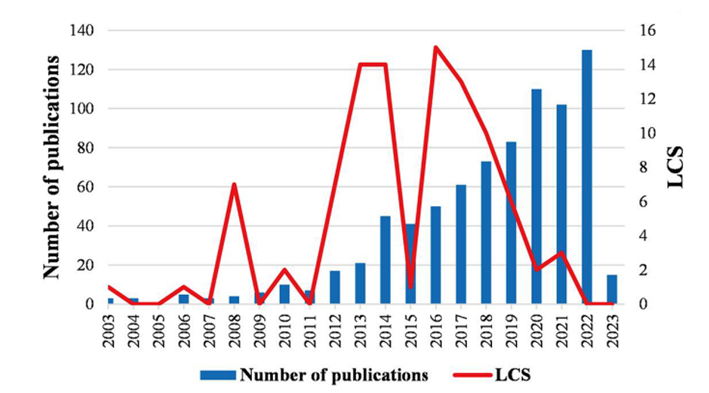
\includegraphics[width=\textwidth]{2/figures/Tendencia.png}
	\caption{Número de publicaciones relacionadas con mHealth. Fuente: \cite{global_trends_mhealth_2023}}
	\label{7:fig}
\end{figure}

Como se aprecia en la Figura N°\ref{7:fig}, el número de publicaciones relacionadas con mHealth ha ido en aumento, especialmente a partir de 2007, mostrando un crecimiento sostenido de más de 100 artículos por año desde 2020. Este incremento se debe, en gran medida, al impulso de la tecnología móvil y el impacto de la pandemia de COVID-19, que aceleró el desarrollo de herramientas de aprendizaje remoto y de salud digital en el ámbito educativo. En los últimos cinco años, la investigación en este campo ha experimentado un auge, con alrededor de 130 artículos nuevos publicados anualmente.
En los siguientes párrafos se detallan los estudios clave sobre mHealth en educación médica, los cuales servirán de base para el planteamiento de teorías y estrategias en el ámbito de la salud digital que se abordarán en este capítulo.


Un primer trabajo corresponde a \parencite{pascucci2021}, donde se desarrolló una aplicación móvil basada en inteligencia artificial (IA) con el objetivo de realizar análisis de resistencia antimicrobiana mediante pruebas de susceptibilidad a antibióticos (AST) en entornos con recursos limitados. La aplicación permite capturar imágenes de antibiogramas usando la cámara de un smartphone y, mediante algoritmos de procesamiento de imágenes y aprendizaje automático, analiza automáticamente las zonas de inhibición alrededor de los discos de antibióticos, proporcionando una interpretación de los resultados.
El objetivo principal fue desarrollar una herramienta móvil accesible y autónoma para realizar análisis de resistencia a antibióticos en entornos con recursos limitados, donde los sistemas de prueba automáticos suelen ser costosos o no están disponibles. La metodología incluyó el uso de algoritmos avanzados para el procesamiento de imágenes, basados en una biblioteca desarrollada en C++ que utiliza OpenCV y TensorFlow. Estos algoritmos permiten detectar y medir las zonas de inhibición en los antibiogramas, identificando los discos de antibióticos y ajustándose a los estándares de clasificación de susceptibilidad. Además, la aplicación cuenta con un sistema experto que evalúa la coherencia de los resultados de los AST, utilizando reglas de interpretación de comités internacionales como el EUCAST (European Committee on Antimicrobial Susceptibility Testing). Este sistema permite interpretar los resultados de manera automatizada, proporcionando diagnósticos y alertas de resistencia.
Para evaluar el rendimiento de la aplicación, se realizaron pruebas con tres conjuntos de datos de antibiogramas. Dos de estos conjuntos (A1 y A2) provenían de un hospital universitario en Créteil, Francia, y consistían en 570 y 75 muestras, respectivamente, procesadas durante la rutina diaria de laboratorio. El tercer conjunto (A3) se generó en un hospital de Médicos Sin Fronteras en Ammán, Jordania, utilizando microorganismos estandarizados de la American Type Culture Collection (ATCC). La precisión de la aplicación se comparó con la lectura manual (considerada estándar de oro) y con sistemas automáticos comerciales. La aplicación mostró una precisión del 90\% en la categorización de susceptibilidad frente a un sistema hospitalario automático y un 98\% en comparación con la medición manual, reduciendo la variabilidad entre operadores. Podemos apreciar mejor estos resultados en la Figura N°\ref{8:fig}

\begin{figure}[ht]
	\centering
	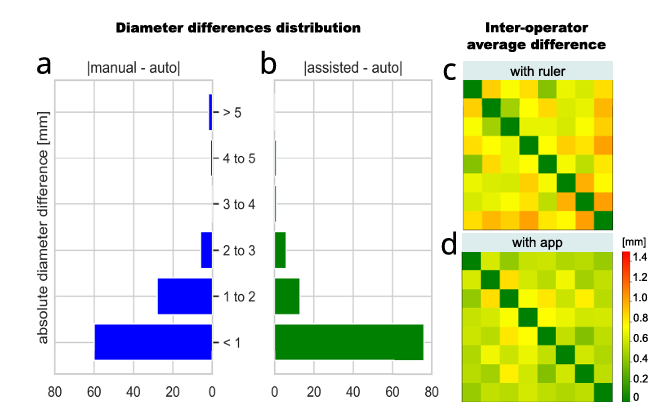
\includegraphics[width=\textwidth]{2/figures/R1.png}
	\caption{Resultados de referencia en el conjunto de datos A3. Los histogramas (a,b) muestran la distribución de las diferencias absolutas de diámetro entre el procedimiento automático de la App (auto) y la medición manual con regla (a), así como con el diámetro ajustado en el teléfono inteligente por los técnicos (asistido, b). A la derecha, los mapas de calor muestran la diferencia de medición absoluta promedio entre los ocho técnicos (dados dos lectores i y j, el cuadrado i, j representa la diferencia promedio entre ellos) que miden con la regla (c) y en modo asistido con la App (d). La medición asistida parece reducir la variabilidad entre operadores.. Fuente: \cite{pascucci2021}}
	\label{8:fig}
\end{figure}

La aplicación emplea estos conjuntos de datos como base de referencia para evaluar y optimizar sus algoritmos de medición de diámetros de inhibición y su sistema de interpretación. Además, el sistema experto contiene una base de conocimiento integrada, actualizada regularmente, que permite interpretar los resultados en función de las reglas de susceptibilidad del EUCAST. Gracias a su diseño offline y su compatibilidad con smartphones básicos, la aplicación resulta adecuada para su uso en áreas con recursos limitados, ampliando el acceso a pruebas de susceptibilidad y apoyando la lucha contra la resistencia antimicrobiana a nivel global.
 
Un segundo trabajo corresponde a \parencite{leung2022}, en el cual se desarrolló un sistema de recomendación basado en procesamiento de lenguaje natural (PLN) para identificar pacientes con cáncer que experimentan desafíos psicosociales y proporcionarles apoyo en el autocuidado a través de grupos de apoyo en línea. El objetivo principal fue implementar un sistema que detecte preocupaciones psicosociales en tiempo real durante las sesiones de grupo y recomiende recursos en línea personalizados para cada paciente, facilitando así el acceso a apoyo sin añadir carga adicional para los terapeutas.
La metodología incluyó el desarrollo de un algoritmo de PLN entrenado con un corpus de aproximadamente 80,000 mensajes de sesiones de apoyo en línea de CancerChatCanada (CCC). Se empleó el modelo Word2Vec para representar palabras en un espacio vectorial, permitiendo identificar expresiones semánticamente similares y extraer preocupaciones de los pacientes. Posteriormente, un sistema de recomendación asignó los recursos más adecuados según el perfil del paciente, tomando en cuenta factores como tipo de cáncer, edad, nivel de participación, síntomas de depresión y ansiedad, y estatus de cuidador. La base de datos de recursos consistió en 37 recursos en línea curados por terapeutas de CCC, evaluados en cuanto a su accesibilidad, relevancia y calidad.
\begin{figure}[ht]
	\centering
	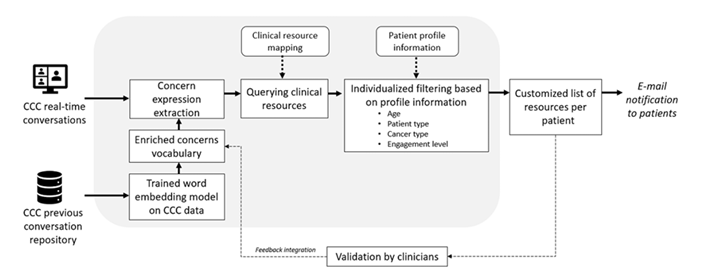
\includegraphics[width=\textwidth]{2/figures/CANADA.png}
	\caption{Descripción general del marco del sistema de recomendación de cofacilitadores basado en inteligencia artificial. CCC: CancerChatCanada. Fuente: \cite{leung2022}}
	\label{9:fig}
\end{figure}

Los resultados del sistema mostraron una alta precisión y capacidad de recuperación. Tras tres rondas de evaluación y mejora, el sistema alcanzó una precisión de 79.7\%, una recuperación de 98.1\% y una puntuación F1 de 88.0\%. De los 48 pacientes a quienes se les recomendaron recursos, el 52\% accedió a al menos un recurso, y el 76\% de estos pacientes encontró los recursos útiles. Estos hallazgos sugieren que el sistema basado en PLN es efectivo para ofrecer apoyo psicosocial personalizado a pacientes de cáncer en grupos de apoyo en línea, aumentando la accesibilidad a recursos relevantes y mejorando la experiencia del paciente en el manejo de sus desafíos emocionales y psicosociales.

Un tercer trabajo corresponde a \parencite{lee2024}, quienes desarrollaron un chatbot de atención médica basado en ChatGPT para proporcionar respuestas médicas precisas a pacientes con cáncer. El objetivo principal de este trabajo fue crear un servicio de chatbot que, mediante modelos de lenguaje natural (LLM), pueda brindar información médica confiable y específica para pacientes oncológicos en tiempo real, abordando las necesidades de información no satisfechas de estos pacientes.
La metodología en la figura N°\ref{9:fig} incluyó la creación de una base de datos especializada en conocimientos médicos sobre cáncer, construida con la colaboración de expertos en oncología. La base de datos integró guías prácticas acreditadas de distintas asociaciones médicas, incluyendo la Red Nacional de Cáncer de los Estados Unidos y la Sociedad Europea de Oncología, resultando en un meta-dataset de 1.17 millones de tokens. Este dataset fue categorizado en áreas como definición, epidemiología, causas, síntomas, diagnóstico, y tratamiento. La implementación del chatbot se realizó utilizando Python, combinando la API de OpenAI y el framework LangChain para facilitar la escalabilidad y permitir interacciones en múltiples idiomas.

\begin{figure}[ht]
	\centering
	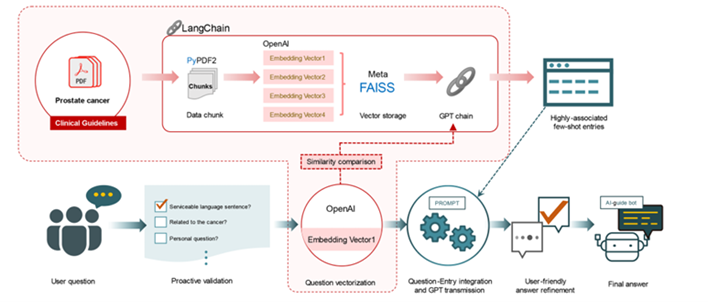
\includegraphics[width=\textwidth]{2/figures/BOT IA.png}
	\caption{Proceso de desarrollo de un bot basado en inteligencia artificial para pacientes con cáncer Fuente: \cite{lee2024}}
	\label{9:fig}
\end{figure}
Para la evaluación del rendimiento, el chatbot fue probado con un conjunto de 100 preguntas relacionadas con el cáncer, seleccionadas y validadas por oncólogos para garantizar respuestas precisas y actualizadas. La precisión, claridad y facilidad de lectura de las respuestas fueron evaluadas usando una escala Likert, donde se obtuvo un puntaje total promedio de 90.98. Estos resultados muestran que el chatbot fue efectivo en comprender las preguntas y en proporcionar respuestas claras y precisas, contribuyendo así a mejorar la accesibilidad de los pacientes a información médica verificada y a reducir la dependencia de fuentes poco confiables en internet.

Un cuarto trabajo corresponde a \parencite{smak2023}, en el cual se desarrolló un estudio piloto de viabilidad para evaluar el uso de una aplicación móvil basada en inteligencia artificial (IA) llamada SkinVision para el diagnóstico de cáncer de piel en el hogar. El objetivo principal de este estudio fue investigar las condiciones y la viabilidad de implementar una aplicación de salud móvil en la atención primaria para detectar lesiones cutáneas sospechosas, facilitando así la atención inicial y reduciendo las consultas innecesarias con médicos generales.
La metodología utilizada fue un diseño de métodos mixtos con la participación de tres prácticas de médicos generales en los Países Bajos. Durante el estudio, se incluyeron 50 pacientes que utilizaron la aplicación para evaluar sus lesiones cutáneas antes de consultar a su médico. La aplicación emplea una red neuronal convolucional para clasificar las fotos de las lesiones cutáneas como de alto o bajo riesgo, sugiriendo a los usuarios de alto riesgo que visiten a su médico. Además, los datos cualitativos fueron recolectados mediante observaciones, diarios de audio y entrevistas con los pacientes y médicos para comprender mejor las experiencias y percepciones del uso de la aplicación.
Los resultados mostraron una tasa de éxito del 84\% en la participación de los pacientes y del 90\% en la de los médicos generales. De los pacientes con lesiones benignas y clasificación de bajo riesgo, el 54\% indicó que se sentiría seguro cancelando su cita con el médico. Aunque la precisión de la aplicación fue alta, no cambió significativamente la precisión diagnóstica de los médicos, aunque en algunos casos influyó en el plan de tratamiento.
Este estudio no menciona una base de datos específica para entrenamiento o evaluación de la aplicación, ya que SkinVision es una aplicación validada y registrada en Europa. Los hallazgos preliminares sugieren que es factible implementar una aplicación basada en IA para la detección de cáncer de piel en entornos de atención primaria, lo que podría reducir la carga en los médicos generales al disminuir las consultas para lesiones benignas.

Un quinto trabajo corresponde a \parencite{jagadish2024}, en el cual se desarrolló una aplicación móvil basada en inteligencia artificial (IA) para ayudar a personas con discapacidad visual. El objetivo principal de esta aplicación fue mejorar la accesibilidad y promover la independencia de las personas con discapacidades visuales, brindándoles información en tiempo real sobre su entorno y facilitando actividades cotidianas.
La metodología incluyó la selección y entrenamiento de algoritmos de IA específicos para cada función de la aplicación, como reconocimiento de objetos, reconocimiento de color, lectura de texto y detección de billetes. Para entrenar estos modelos se utilizaron conjuntos de datos relevantes, como imágenes de objetos y colores, datos de texto para lectura de billetes y códigos de barras, y modelos preentrenados en TensorFlow Lite. La aplicación se desarrolló para funcionar en dispositivos Android, integrando características como comandos de voz, modos de alto contraste y compatibilidad con lectores de pantalla para garantizar la accesibilidad.
Los resultados demostraron que la aplicación puede reconocer y describir objetos, identificar colores en tiempo real, leer texto en voz alta y detectar billetes, ofreciendo así una experiencia más autónoma y segura para los usuarios con discapacidad visual. La interfaz fue diseñada para ser intuitiva y accesible, con retroalimentación táctil y compatibilidad con comandos de voz. El sistema funciona de manera offline, lo que permite su uso en áreas con conectividad limitada.
Este trabajo no menciona una base de datos específica para almacenar datos de los usuarios o resultados de detección; sin embargo, utiliza conjuntos de datos de entrenamiento y modelos preentrenados para lograr la funcionalidad de reconocimiento y descripción en tiempo real. Este proyecto resalta el potencial de las aplicaciones móviles basadas en IA para mejorar la accesibilidad y calidad de vida de personas con discapacidades visuales.

Un sexto trabajo corresponde a \parencite{khan2020}, quienes realizaron una revisión sistemática sobre la aplicación de inteligencia artificial (IA) y análisis de big data en el ámbito de la salud móvil (m-health), con el objetivo de identificar cómo estas tecnologías pueden mejorar los sistemas de atención médica. Este estudio tuvo como objetivo principal evaluar las aplicaciones actuales de IA y big data en m-health y proponer un modelo que optimice el uso de estas tecnologías para enfrentar desafíos específicos en la salud móvil.

La metodología empleada consistió en una revisión sistemática de artículos científicos, recopilando 106 estudios relevantes de bases de datos como IEEE Xplore, ACM Digital Library y ScienceDirect. Los artículos seleccionados abordan aplicaciones de IA y big data en salud móvil, utilizando criterios de inclusión y exclusión basados en el uso de estas tecnologías en el monitoreo de salud, diagnóstico y análisis de datos médicos. Se utilizó el diagrama de flujo Prisma como se ve en la figura N°\ref{10:fig} para el proceso de revisión.

\begin{figure}[H]
	\centering
	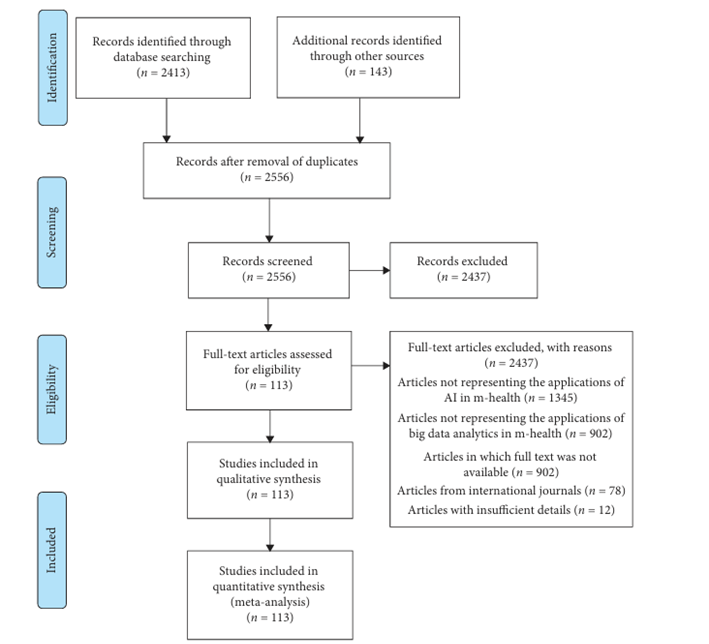
\includegraphics[width=\textwidth]{2/figures/PRISMA.png}
	\caption{Diagrama de Flujo Prisma para el proceso de revisión de artículos. Fuente: \cite{khan2020}}
	\label{10:fig}
\end{figure}



Los resultados de esta revisión destacaron aplicaciones de IA para el análisis de datos de salud, como el uso de sensores móviles para monitorear condiciones físicas y mentales, así como la implementación de modelos de aprendizaje automático para mejorar la precisión en el diagnóstico. Se propuso un modelo basado en IA y big data para m-health (ver figura N°\ref{11:fig}), que incluye la recolección de datos mediante dispositivos móviles, el análisis de big data, y una plataforma para la toma de decisiones en tiempo real.

\begin{figure}[H]
	\centering
	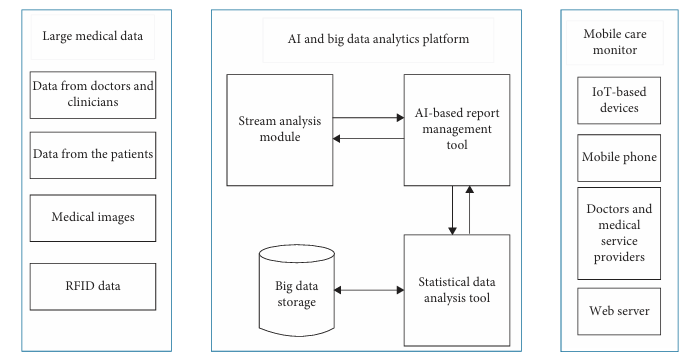
\includegraphics[width=\textwidth]{2/figures/MODELO.png}
	\caption{Modelo basado en IA y big data para m-health. Fuente: \cite{khan2020}}
	\label{11:fig}
\end{figure}

\vspace{0.5 cm}
Este estudio no emplea una base de datos específica, pero sugiere el uso de grandes volúmenes de datos médicos provenientes de registros electrónicos de salud (EHRs), imágenes médicas y otros datos clínicos para optimizar el m-health. Los hallazgos subrayan el potencial de la IA y el big data para mejorar la calidad de los sistemas de m-health, facilitando el acceso a información en tiempo real y mejorando la toma de decisiones clínicas.







Un séptimo  trabajo corresponde a \parencite{prevljak2024}, en el cual se exploró la aplicación de inteligencia artificial (IA) en la detección de cáncer de mama y en el monitoreo de resultados de laboratorio. El objetivo principal de este estudio fue mejorar la precisión y velocidad en el diagnóstico temprano del cáncer de mama, utilizando IA para analizar imágenes médicas y biomarcadores, lo cual contribuiría a una detección temprana y a reducir la tasa de resultados falsos negativos.
La metodología incluyó una revisión exhaustiva de 60 artículos científicos sobre la implementación de IA en la investigación del cáncer de mama, con datos recopilados de bases de datos como PubMed. El estudio analizó técnicas de aprendizaje profundo, especialmente redes neuronales convolucionales (CNN), aplicadas en el procesamiento de imágenes de mamografía, MRI y PET-CT, así como el análisis de biomarcadores. Los algoritmos de IA fueron entrenados para identificar patrones sutiles y anormalidades en imágenes médicas, ayudando a los profesionales en la toma de decisiones clínicas.
Los resultados del estudio indicaron que el uso de CNN y otras técnicas de IA en el análisis de imágenes aumentó significativamente la precisión en la detección de cáncer de mama en etapas tempranas. La IA también permitió la evaluación de biomarcadores como HER2 y Ki-67, mejorando la capacidad de personalizar los tratamientos según las características individuales del paciente. Estos hallazgos subrayan el potencial de la IA para transformar el diagnóstico y tratamiento del cáncer de mama, optimizando la toma de decisiones y mejorando los resultados en pacientes.


Un octavo antecedente corresponde al desarrollo de MentalApp, una aplicación móvil creada para facilitar el seguimiento del bienestar mental mediante herramientas personalizadas, tales como encuestas, sensores y comunicación directa con profesionales de la salud. Este proyecto fue llevado a cabo por un equipo de estudiantes de la Pontificia Universidad Javeriana y su propósito principal es brindar soporte a los usuarios en la gestión de su salud mental de una forma accesible y eficiente. La meta del proyecto fue migrar una plataforma web de salud mental a una aplicación móvil, con el fin de mejorar la accesibilidad y usabilidad para los usuarios jóvenes, ofreciendo un seguimiento y monitoreo más exhaustivo de su bienestar mental. 
La aplicación busca registrar y evaluar aspectos como el estado emocional, el estrés, el sueño y otros indicadores de salud mental, brindando recursos personalizados y acceso a profesionales de la salud. (Propuesta de solución Figura N°\ref{12:fig})

\begin{figure}[ht]
	\centering
	\includegraphics[width=\textwidth]{2/figures/PROPUESTA DE SOLUCIÓN.png}
	\caption{Propuesta de solución. Fuente: \cite{coral2023}}
	\label{12:fig}
\end{figure}

Para el desarrollo de MentalApp, se utilizó un enfoque de metodologías ágiles, combinando Scrum y Sawtooth. Esta elección metodológica permitió dividir las tareas en sprints con retroalimentación constante de los interesados. La estructura de la aplicación se fundamentó en una arquitectura en capas (Layered Pattern), que organiza la lógica de negocios, la integración, la presentación y el modelo de dominio. En cuanto a las herramientas utilizadas, el equipo empleó Flutter para el desarrollo de la interfaz, Java y Spring Boot para los servicios de backend, y MySQL como sistema de gestión de bases de datos. Además, se integró Jitsi Meet para permitir videollamadas. La aplicación incluyó también el uso de sensores mediante la integración de la API de reconocimiento de actividad (Activity Recognition API) de Android para monitorear actividades físicas de los usuarios. Sin embargo, debido a las políticas de Google Play Store, la recopilación de datos del GPS se limitó a situaciones en las que la aplicación se ejecutaba en primer plano. Para asegurar el correcto funcionamiento del sistema antes de la versión Alpha, se realizaron pruebas de componentes y evaluaciones en sprints. Asimismo, se llevaron a cabo encuestas de satisfacción con usuarios para evaluar la facilidad de uso y la utilidad de la aplicación. La implementación de todo esto se puede apreciar en la figura N°\ref{13:fig}

\begin{figure}[ht]
	\centering
	\includegraphics[width=\textwidth]{2/figures/IMPLEMENTACIÓN MENTALAPP.png}
	\caption{Implementación MentalAPP. Fuente: \cite{coral2023}}
	\label{13:fig}
\end{figure}

Entre los componentes principales de MentalApp, se encuentran las encuestas periódicas, que permiten a los usuarios completar evaluaciones sobre distintos aspectos de su salud mental, como el estrés, el sueño y el bienestar emocional. La aplicación también incluye un plan de bienestar que permite a los usuarios registrar actividades, crear contactos de emergencia y gestionar signos de alarma, ofreciendo un seguimiento personalizado de su estado de salud mental. Otra funcionalidad importante es la comunicación directa con profesionales de la salud, donde los usuarios pueden solicitar orientación mediante chat o videollamadas, accediendo así a apoyo psicológico en tiempo real. Además, MentalApp ofrece recursos personalizados a los usuarios, como artículos y recomendaciones específicas de acuerdo con sus necesidades, propuestas por profesionales de la salud.
Las pruebas de usuario revelaron que los participantes encontraron la aplicación fácil de entender, intuitiva y satisfactoria en términos de experiencia de usuario. Estos resultados también indicaron una alta probabilidad de recomendación de la aplicación, lo que sugiere un impacto positivo en su aceptación general. MentalApp utiliza tres bases de datos relacionales en MySQL, cada una con un propósito específico: RegisterDB, que contiene los datos de los usuarios, incluyendo su historial médico y registros de orientación; SurveyDB, que almacena los resultados de las encuestas y los datos obtenidos de los sensores; y BotnarDB, que gestiona los planes de bienestar y las relaciones entre los usuarios y los profesionales de la salud. Este antecedente demuestra cómo una aplicación móvil puede ser una herramienta eficaz en el monitoreo y apoyo a la salud mental, especialmente en poblaciones jóvenes que enfrentan barreras de acceso a servicios de salud mental. MentalApp facilita el seguimiento de indicadores clave de bienestar y permite a los usuarios recibir recomendaciones personalizadas y apoyo profesional de manera accesible y conveniente.


\section{Bases Teóricas}
\subsection{Aplicaciones móviles }
Las aplicaciones móviles son programas diseñados específicamente para ejecutarse en dispositivos móviles como teléfonos inteligentes y tabletas. Estas aplicaciones, que pueden variar en funcionalidad, incluyen desde entretenimiento hasta educación y salud, y permiten a los usuarios acceder a información y servicios de manera rápida y eficiente. Según \parencite{herazo2023}, una aplicación móvil es un tipo de software que se descarga y utiliza en un dispositivo móvil, que puede ser un smartphone o una tablet, y que facilita la realización de tareas específicas o la interacción con servicios y contenidos en línea en varios. Se pueden clasificar en tres categorías principales:

Se pueden clasificar en tres categorías principales:

\begin{itemize}
    \item \textbf{Aplicaciones nativas}: Están desarrolladas para un sistema operativo específico, como Android o iOS. Al estar diseñadas para una plataforma específica, las aplicaciones nativas ofrecen un rendimiento óptimo y una integración completa con el hardware y las funcionalidades del dispositivo.
    
    \item \textbf{Aplicaciones web}: Estas aplicaciones son accesibles a través de navegadores web y se ejecutan directamente en el navegador del dispositivo, lo que permite que sean multiplataforma. Aunque no requieren instalación y pueden funcionar en cualquier dispositivo, su rendimiento y funcionalidad pueden estar limitados en comparación con las aplicaciones nativas.
    
    \item \textbf{Aplicaciones híbridas}: Son una combinación de aplicaciones nativas y web, desarrolladas con tecnologías como React Native o Flutter, y permiten compartir gran parte de su código entre plataformas. Las aplicaciones híbridas ofrecen una experiencia similar a las aplicaciones nativas, pero con un menor costo de desarrollo y mantenimiento al utilizar una única base de código.
\end{itemize}

 \subsection{Inteligencia artificial}

 La inteligencia artificial (IA) es una disciplina de la informática dedicada a desarrollar sistemas capaces de realizar tareas que, en condiciones normales, requerirían inteligencia humana. Entre estas tareas se incluyen el reconocimiento de patrones, la toma de decisiones y el aprendizaje. \parencite{russell2004} definen la IA como el estudio de los agentes que perciben su entorno y toman acciones que maximizan sus posibilidades de éxito en alguna tarea.
En el ámbito de la salud, la IA se aplica en el análisis de grandes volúmenes de datos clínicos, lo que permite a los sistemas identificar patrones que facilitan el diagnóstico y la personalización de tratamientos. Según Google, la IA generativa, una subrama de la IA, permite a los modelos crear contenido nuevo a partir de datos existentes, lo cual es especialmente útil para generar imágenes médicas sintéticas y para la creación de asistentes virtuales que interactúan con los pacientes de forma personalizada \parencite{googlecloud2023}.

\subsubsection{Inteligencia artificial generativa}:

La IA generativa se enfoca en la creación de nuevo contenido a partir de patrones aprendidos en datos previos. Esta tecnología es capaz de generar textos, imágenes y otros tipos de contenido que imitan los patrones de los datos originales, lo cual la hace valiosa en aplicaciones médicas, especialmente en la creación de datos sintéticos para entrenar otros sistemas de IA. La plataforma de Google Cloud destaca que esta tecnología puede asistir en "la creación de asistentes virtuales en aplicaciones de salud" para apoyar a los pacientes y brindar soporte emocional en tiempo real \parencite{googlecloud2023} .

\subsection{Aprendizaje automático}

El aprendizaje automático (machine learning) es una técnica de IA que permite a los sistemas aprender de los datos sin una programación explícita para cada tarea específica. En lugar de ser programados con instrucciones precisas, estos sistemas emplean algoritmos que procesan datos y mejoran sus predicciones o clasificaciones a medida que aprenden de ejemplos previos. Según Oracle, el aprendizaje automático se basa en tres enfoques principales: el aprendizaje supervisado, no supervisado y por refuerzo, y cada uno tiene aplicaciones específicas en el diagnóstico y análisis de datos médicos \parencite{oracle2023}.

\subsection{Procesamiento del lenguaje natural}

El procesamiento del lenguaje natural (PLN) es una rama de la IA que permite a los sistemas entender y generar lenguaje humano de manera comprensible. En el contexto de la salud, el PLN es utilizado para desarrollar chatbots y asistentes virtuales que pueden interactuar con los pacientes de forma empática y personalizada, respondiendo a sus preguntas y brindando apoyo emocional. IBM define el PLN como "la tecnología que permite a las computadoras procesar y analizar grandes cantidades de lenguaje humano" y señala que esta capacidad es esencial para mejorar la experiencia del paciente en aplicaciones de soporte emocional y salud \parencite{ibm2023} .

\subsection{Base de datos}:
Las bases de datos son sistemas que permiten almacenar, gestionar y recuperar grandes volúmenes de información de manera eficiente, poseen una estructura definida y representan entidades y las relaciones que existen entre ellas. Estas bases de datos o repositorios contienen información ordenada que puede ser consultada a través de diversos usuarios \parencite{perez2007}. Una base de datos puede definirse como "un sistema organizado de almacenamiento de datos que permite la administración, la seguridad y el acceso rápido a los datos" \parencite{nutanix2023}.

Las bases de datos se caracterizan por ofrecer:
\begin{itemize}
    \item \textbf{Organización estructurada}: Los datos se organizan en tablas compuestas por columnas y filas, lo que permite una categorización y recuperación de la información de manera rápida y eficiente.
    \item \textbf{Reducción de redundancia}: Las bases de datos están diseñadas para minimizar la duplicidad de datos, asegurando que cada pieza de información se almacene solo una vez.
    \item \textbf{Consultas complejas}: Permiten realizar búsquedas avanzadas, consultas y análisis de datos a través de lenguajes de consulta como SQL (Structured Query Language), lo que facilita la obtención de información específica dentro de grandes volúmenes de datos.
    \item \textbf{Seguridad y control de acceso}: Implementan medidas de seguridad que controlan el acceso a los datos, permitiendo que solo usuarios autorizados puedan visualizar o modificar la información.
    \item \textbf{Recuperación y respaldo}: Las bases de datos suelen contar con mecanismos de respaldo y recuperación, lo que garantiza que la información esté protegida contra posibles fallos.
\end{itemize}

Para construir una base de datos, se diseña un modelo de datos en el cual se identifican las entidades clave, las relaciones entre ellas y los atributos de cada entidad. Este proceso permite definir la estructura de la base de datos, optimizando la organización y el acceso a la información. Existen varios tipos de relaciones en una base de datos:
\begin{itemize}
    \item \textbf{Relación de uno a uno}: Cada registro en la tabla A se asocia con un único registro en la tabla B. Por ejemplo, una persona y su número de pasaporte.
    \item \textbf{Relación de uno a muchos}: Un registro en la tabla A puede estar vinculado a múltiples registros en la tabla B. Un ejemplo sería un cliente que tiene varios pedidos asociados.
    \item \textbf{Relación de muchos a muchos}: Los registros en la tabla A pueden estar vinculados con múltiples registros en la tabla B y viceversa, como estudiantes que pueden estar inscritos en varios cursos, y cursos que pueden tener varios estudiantes inscritos.
\end{itemize}

El diseño adecuado de estas relaciones es esencial para asegurar la eficiencia y escalabilidad de la base de datos, especialmente en aplicaciones de gran tamaño y con requisitos de rendimiento elevados \parencite{nutanix2023}.

\subsubsection{Base de datos no relacionadas}

Las bases de datos no relacionales, también conocidas como bases de datos NoSQL, se diferencian de las bases de datos relacionales en que no emplean un esquema de tablas tradicional y no necesitan seguir una estructura rígida de filas y columnas. Este tipo de bases de datos es particularmente útil para el almacenamiento de datos no estructurados o semiestructurados, como archivos multimedia, documentos y datos de sensores, donde la flexibilidad es esencial. Según el blog de FP Superior UFV, las bases de datos no relacionales "permiten almacenar datos de una forma más flexible y escalable, siendo ideales para manejar grandes volúmenes de información en tiempo real" \parencite{fpsuperiorufv2023}.


Existen varios tipos de bases de datos no relacionales, cada uno con una estructura específica adaptada a diferentes casos de uso:
\begin{itemize}
    \item \textbf{Bases de datos de documentos}: Organizan los datos en formato de documentos, como JSON o XML, donde cada documento contiene una estructura única y flexible que se adapta a la información específica de cada registro.
    \item \textbf{Bases de datos de clave-valor}: Almacenan datos en pares de clave y valor, permitiendo una búsqueda rápida basada en una clave única. Este tipo de base es adecuado para aplicaciones que requieren almacenamiento de datos sencillo y de rápido acceso.
    \item \textbf{Bases de datos de grafos}: Emplean nodos y aristas para representar relaciones entre entidades, siendo ideales para analizar redes sociales o sistemas de recomendaciones.
    \item \textbf{Bases de datos de columnas}: Organizan los datos en columnas en lugar de filas, lo cual mejora el rendimiento en consultas analíticas de gran escala.
\end{itemize}

En aplicaciones de salud, las bases de datos no relacionales ofrecen una gran flexibilidad y escalabilidad, permitiendo manejar datos complejos y variados, como registros de pacientes, datos de dispositivos de monitoreo en tiempo real y grandes volúmenes de información generados por sistemas de inteligencia artificial. Amazon Web Services (AWS) destaca que las bases de datos NoSQL permiten manejar "grandes cantidades de datos y realizar consultas rápidas y escalables", lo que es esencial para aplicaciones que requieren respuestas en tiempo real \parencite{aws2023}.

Microsoft Azure, en su guía de arquitectura de datos, también señala que las bases de datos no relacionales son particularmente efectivas en entornos de big data, donde los datos se generan rápidamente y en formatos variados. Este tipo de bases de datos es adecuado para escenarios donde el esquema puede evolucionar con el tiempo y no es necesario seguir una estructura fija como en las bases de datos relacionales \parencite{microsoft2023}.

La flexibilidad de las bases de datos no relacionales las convierte en una opción ideal para aplicaciones móviles de salud, donde se requiere un almacenamiento rápido y dinámico que permita adaptarse a las necesidades cambiantes de los usuarios y los datos médicos que se recogen continuamente.

\subsection{Cáncer}

El cáncer es un conjunto de enfermedades caracterizadas por el crecimiento descontrolado y la propagación de células anormales en el organismo. Según el Instituto Nacional del Cáncer, el cáncer "puede comenzar en casi cualquier parte del cuerpo y es causado por cambios en los genes que regulan el crecimiento y la división celular" \parencite{institutonacionalcancer2023}. Las células cancerosas tienen la capacidad de invadir tejidos adyacentes y pueden diseminarse a otras partes del cuerpo a través del sistema linfático o el torrente sanguíneo en un proceso conocido como metástasis.

La Organización Mundial de la Salud (OMS) señala que el cáncer es una de las principales causas de muerte en el mundo, con aproximadamente 10 millones de muertes al año. Entre los factores de riesgo de desarrollar cáncer se incluyen el consumo de tabaco, la falta de actividad física, la dieta poco saludable y el consumo excesivo de alcohol. La OMS enfatiza la importancia de la detección temprana y del tratamiento oportuno para mejorar las tasas de supervivencia de los pacientes \parencite{oms2023}.

\subsubsection{Cáncer de Mama}

El cáncer de mama es uno de los tipos de cáncer más comunes en mujeres y es la principal causa de muerte por cáncer en este grupo a nivel mundial. El cáncer de mama se desarrolla cuando las células de la mama comienzan a crecer de manera descontrolada, formando un tumor que puede ser benigno o maligno. Según la Mayo Clinic, "el cáncer de mama puede aparecer en hombres y mujeres, pero es mucho más frecuente en las mujeres" \parencite{mayoclinic2023}.

Los síntomas del cáncer de mama incluyen:
\begin{itemize}
    \item Un bulto o engrosamiento en el seno que se siente diferente al tejido circundante.
    \item Cambios en el tamaño, forma o apariencia de la mama.
    \item Secreción anormal del pezón, que puede ser sanguinolenta.
    \item Dolor en la mama o el pezón.
    \item Cambios en la piel del seno, como enrojecimiento o formación de hoyuelos.
\end{itemize}

La detección temprana es crucial para mejorar el pronóstico en los casos de cáncer de mama. La autoexploración, las mamografías y los exámenes clínicos de mama son herramientas esenciales en la detección temprana de esta enfermedad.

\subssection{Psicología en Pacientes Oncológicos}

El diagnóstico y tratamiento del cáncer tienen un impacto significativo en la salud emocional y mental de los pacientes. La psicología oncológica, o psicooncología, es una especialidad que aborda las necesidades emocionales de las personas que enfrentan el cáncer, proporcionando herramientas para ayudarles a gestionar el miedo, la ansiedad y la depresión que pueden surgir en el proceso. Según Oncosalud, "el psicólogo cumple un rol fundamental en el tratamiento del cáncer, ayudando al paciente a afrontar los retos emocionales y psicológicos que acompañan a la enfermedad" \parencite{oncosalud2023}.

El apoyo psicológico en pacientes con cáncer no solo beneficia al paciente, sino también a sus familiares, quienes también pueden experimentar un gran estrés emocional debido a la enfermedad de su ser querido. La intervención psicológica puede mejorar la calidad de vida del paciente, ayudándole a mantener una actitud positiva frente a los tratamientos y a reducir los síntomas de depresión y ansiedad. De acuerdo con Área Humana, "el apoyo psicológico a los pacientes oncológicos permite a estos sentirse acompañados en su proceso, lo que ayuda a disminuir la angustia y a mejorar su bienestar general" \parencite{areahumana2023}.

La psicooncología incluye diversas técnicas y terapias adaptadas a las necesidades de cada paciente. Algunas de estas incluyen la terapia cognitivo-conductual, que ayuda a los pacientes a identificar y modificar pensamientos negativos, y la terapia de aceptación y compromiso, que se centra en aceptar la realidad de la enfermedad y trabajar en objetivos de vida significativos. Terapify menciona que "el tratamiento psicológico para pacientes con cáncer, conocido como psicooncología, se adapta a cada fase de la enfermedad, proporcionando apoyo en el diagnóstico, durante el tratamiento y en la recuperación" \parencite{terapify2023}.


\subsection{Desarrollo de Aplicaciones Móviles}

El desarrollo de aplicaciones móviles es el proceso de creación de software diseñado para ejecutarse en dispositivos móviles, como teléfonos inteligentes y tabletas. Este proceso involucra varias etapas, desde la concepción de la idea hasta el diseño, desarrollo, pruebas y despliegue de la aplicación en las tiendas de aplicaciones. Según Mathew y Clark Kimberly, "el desarrollo de aplicaciones móviles es el conjunto de procesos y procedimientos que implican la escritura de software para dispositivos inalámbricos pequeños, como teléfonos inteligentes y otros dispositivos portátiles" \parencite{mathew2023}. El desarrollo de aplicaciones móviles puede dividirse en tres tipos principales: desarrollo de aplicaciones nativas, híbridas y web, cada uno de los cuales ofrece diferentes ventajas y desafíos en términos de rendimiento, compatibilidad y costos de desarrollo.

\subsubsection{Desarrollo de Aplicaciones Móviles en la Salud}

El desarrollo de aplicaciones móviles para el sector salud ha crecido significativamente en los últimos años, proporcionando herramientas innovadoras para mejorar el acceso a la atención médica y el monitoreo de la salud de los pacientes. Estas aplicaciones permiten a los profesionales de la salud y a los pacientes acceder a información y servicios de manera rápida y conveniente, lo cual ha transformado el sistema de atención sanitaria. De acuerdo con Reanima Soluciones, las aplicaciones móviles de salud "brindan acceso a servicios médicos, permiten el monitoreo de pacientes y facilitan la recopilación y análisis de datos médicos en tiempo real" \parencite{reanima2023}.

Las aplicaciones de salud ofrecen funcionalidades como la consulta en línea, la gestión de citas, el monitoreo de signos vitales y el acceso a historiales médicos, lo cual permite una atención más eficiente y personalizada. Para desarrollar una aplicación de salud efectiva, es crucial seguir ciertos pasos, como definir los objetivos de la app, seleccionar las herramientas adecuadas para el desarrollo y cumplir con las normativas de seguridad y privacidad de datos. Según GooApps, una guía completa para el desarrollo de una aplicación de salud debe incluir "la definición de funcionalidades, la selección de tecnologías apropiadas y la validación de la app mediante pruebas exhaustivas para asegurar su usabilidad y seguridad" \parencite{gooapps2022}.

El desarrollo de aplicaciones móviles en el ámbito de la salud no solo ha mejorado la accesibilidad a la atención médica, sino que también ha permitido un seguimiento continuo y en tiempo real de los pacientes, especialmente aquellos con enfermedades crónicas. Este tipo de aplicaciones ha demostrado ser eficaz en la gestión de enfermedades, el seguimiento de tratamientos y la promoción de hábitos saludables, permitiendo una atención más cercana y un control personalizado de la salud del paciente.

\subsection{Herramientas de Desarrollo de Aplicaciones Móviles: Android Studio y Swift}

El desarrollo de aplicaciones móviles requiere herramientas especializadas que permitan crear aplicaciones eficientes, seguras y adaptadas a diferentes plataformas. Android Studio y Swift son dos de las herramientas más populares y utilizadas para el desarrollo de aplicaciones móviles, especialmente en sistemas operativos como Android e iOS, respectivamente.

\subsubsection{Android Studio}

Android Studio es el entorno de desarrollo integrado (IDE) oficial de Google para el desarrollo de aplicaciones en el sistema operativo Android. Lanzado en 2013, Android Studio proporciona una serie de herramientas que permiten a los desarrolladores crear, probar y depurar aplicaciones de manera eficiente. Entre sus características principales, Android Studio incluye un editor de código avanzado, un emulador de dispositivos, y un sistema de gestión de versiones que facilita el control de cambios en el desarrollo del software. Según Developer Android, Android Studio está diseñado para "ofrecer las herramientas más rápidas para la creación de aplicaciones en todos los tipos de dispositivos Android" \parencite{developerandroid2023}.

Android Studio está basado en IntelliJ IDEA y permite programar principalmente en Java y Kotlin, dos lenguajes compatibles con Android. Jesús Santaella (2023) destaca que Android Studio "cuenta con características avanzadas como un editor visual para el diseño de interfaces de usuario, un emulador rápido y una herramienta de análisis de rendimiento", lo cual permite optimizar la experiencia del usuario en aplicaciones móviles \parencite{santaella2023}.

\subsubsection{Swift}

Swift es un lenguaje de programación desarrollado por Apple en 2014 para la creación de aplicaciones en sistemas operativos como iOS, macOS, watchOS y tvOS. Este lenguaje es moderno, seguro y rápido, diseñado para ser fácil de aprender y de usar. Swift permite a los desarrolladores escribir código de manera eficiente y con un rendimiento optimizado, lo cual es crucial para el desarrollo de aplicaciones móviles. Apple describe Swift como "un lenguaje de programación potente e intuitivo para macOS, iOS, watchOS y tvOS, que permite escribir código más seguro y mejorar el rendimiento de las aplicaciones" \parencite{apple2023}.

Swift está diseñado para ser intuitivo y flexible, y es compatible con el marco de trabajo Xcode, el IDE oficial de Apple para el desarrollo de aplicaciones. Según Esteban Fernández (2023), Swift se caracteriza por su sintaxis sencilla y su enfoque en la seguridad, lo cual "reduce errores comunes y mejora la estabilidad de las aplicaciones, especialmente en plataformas móviles" \parencite{fernandez2023}.

Ambas herramientas, Android Studio y Swift, son esenciales para el desarrollo de aplicaciones móviles en sus respectivos sistemas operativos y permiten a los desarrolladores crear aplicaciones optimizadas y personalizadas para mejorar la experiencia del usuario en dispositivos móviles.


\section{Marco Conceptual}
A continuación, se presentan los principales conceptos a utilizar en el presente trabajo de 
investigación.

\begin{itemize}
    \item \textbf{Inteligencia Artificial (IA)} \\
    La inteligencia artificial es una rama de las ciencias computacionales que busca emular la inteligencia humana a través de algoritmos; máquinas y sistemas realizan actividades de manera eficiente, ayudando a resolver problemas complejos en diversos campos, incluido el de la salud. \parencite{russell2004}

    \item \textbf{Machine Learning (Aprendizaje Automático)} \\
    El aprendizaje automático es una subrama de la inteligencia artificial que utiliza estadísticas e ingeniería para permitir que las máquinas mejoren su rendimiento en tareas específicas mediante el aprendizaje de datos. Se utiliza en aplicaciones de salud para analizar datos médicos y mejorar diagnósticos. \parencite{harrington2012}

    \item \textbf{Aprendizaje Supervisado} \\
    Este método de aprendizaje implica la identificación de patrones en los datos basados en un conjunto de entrenamiento etiquetado, donde los resultados esperados están presentes. Es fundamental en el desarrollo de modelos de predicción en aplicaciones de salud. \parencite{harrington2012}
    
    \item \textbf{Aplicaciones Móviles} \\
    Las aplicaciones móviles son programas diseñados para ejecutarse en dispositivos móviles como teléfonos inteligentes y tabletas. Estas aplicaciones pueden clasificarse en tres tipos principales: nativas, híbridas y web, cada una con sus propias ventajas en términos de rendimiento y compatibilidad. \parencite{herazo2023}

    \item \textbf{Desarrollo de Aplicaciones Móviles} \\
    Es el proceso de creación de software diseñado para ejecutarse en dispositivos móviles como teléfonos inteligentes y tabletas, pasando por varias etapas como diseño, desarrollo y pruebas. \parencite{mathew2023}

    \item \textbf{Aplicaciones Móviles en Salud} \\
    Las aplicaciones móviles en el sector salud permiten a los pacientes y profesionales acceder a información y servicios de manera ágil, facilitando el monitoreo y la gestión de la salud. \parencite{reanima2023}

    \item \textbf{Android Studio} \\
    Es el entorno de desarrollo integrado (IDE) oficial de Google para la creación de aplicaciones en Android, lanzado en 2013. Android Studio ofrece herramientas avanzadas como un emulador de dispositivos y un editor visual para optimizar el proceso de desarrollo. \parencite{developerandroid2023, santaella2023}

    \item \textbf{Swift} \\
    Swift es un lenguaje de programación creado por Apple en 2014 para el desarrollo de aplicaciones en sus plataformas como iOS y macOS. Este lenguaje se caracteriza por su seguridad y rendimiento optimizado, ideal para el desarrollo de aplicaciones móviles en salud. \parencite{apple2023, fernandez2023}

    \item \textbf{Cáncer} \\
    El cáncer es un conjunto de enfermedades caracterizadas por el crecimiento descontrolado de células anormales. Puede desarrollarse en cualquier parte del cuerpo y propagarse a través del sistema linfático o sanguíneo. \parencite{institutonacionalcancer2023}

    \item \textbf{Cáncer de Mama} \\
    Tipo de cáncer que afecta principalmente a las mujeres y es uno de los más comunes. Se desarrolla cuando las células de la mama crecen de manera descontrolada, formando un tumor. Los síntomas incluyen bultos en el seno, cambios en la forma y dolor. \parencite{mayoclinic2023}

    \item \textbf{Psicología en Pacientes Oncológicos} \\
    La psicooncología es una especialidad que se enfoca en el apoyo psicológico para pacientes con cáncer, ayudándoles a manejar el estrés, la ansiedad y la depresión asociados al diagnóstico y tratamiento. \parencite{oncosalud2023, areahumana2023, terapify2023}

    \item \textbf{Base de Datos} \\
    Sistema que permite almacenar y gestionar información de manera estructurada, facilitando su recuperación y análisis. Las bases de datos médicas son esenciales en aplicaciones de salud para manejar grandes volúmenes de información clínica. \parencite{perez2007, nutanix2023}



\end{itemize}


\chapter{METODOLOGÍA DE LA INVESTIGACIÓN}

En este capítulo se describe la metodología empleada en el desarrollo de la investigación. Se detallan el diseño de investigación, tipo y enfoque, así como el alcance del estudio. Además, se presentan las estrategias para la recolección y análisis de datos, orientadas a evaluar la efectividad de una aplicación móvil basada en Inteligencia Artificial generativa para el soporte integral a pacientes con cáncer de mama.

\section{Diseño, tipo y enfoque de la investigación}

\subsection{Diseño}

El diseño de la investigación es de tipo experimental, dado que se busca analizar la interacción de los pacientes con la aplicación móvil y evaluar los cambios en su estado de salud y bienestar. Este diseño permite observar los efectos directos del uso de la tecnología en un entorno controlado, mediante la implementación de pruebas piloto en condiciones reales. El nivel de la investigación es explicativo, ya que tiene como objetivo establecer relaciones causales entre el uso de la aplicación y la mejora en el soporte integral ofrecido a los pacientes. Se busca determinar si el empleo de IA generativa en la aplicación contribuye significativamente al monitoreo, control y soporte emociona.

\subsection{Enfoque}
El enfoque adoptado es cuantitativo, lo que permite medir objetivamente variables como la adherencia al tratamiento, la precisión de las predicciones generadas por la IA y la satisfacción del usuario. Este enfoque se sustenta en la recolección de datos numéricos para su posterior análisis estadístico

\subsection{Alcance de la investigación}
El alcance de este estudio se centra en identificar y explicar la relación entre el uso de la aplicación móvil y la mejora en el soporte integral a pacientes con cáncer de mama. La investigación tiene un propósito explicativo, ya que busca profundizar en cómo la tecnología puede impactar positivamente en la experiencia de los pacientes, tanto en aspectos físicos como emocionales

\section{Población y muestra}

\subsection{Población}
La población objetivo de este estudio está conformada por mujeres diagnosticadas con cáncer de mama en etapa temprana o avanzada, que se encuentren en tratamiento en hospitales públicos, clínicas privadas, o que, de manera independiente, deseen participar en el estudio. Esto abarca pacientes de diversas condiciones socioeconómicas y niveles de acceso a servicios de salud en Lima, Perú.
\subsection{Muestra}

El muestreo será no probabilístico por conveniencia, enfocado en mujeres que cumplan con los criterios de inclusión y que voluntariamente acepten participar. Esto permitirá evaluar la efectividad de la aplicación en diversos contextos y niveles de acceso a la atención médica. Donde la muestra estará compuesta entre 5 a 15 pacientes con cáncer de mama por la complejidad de la enfermedad, quienes serán seleccionadas a través de las siguientes vías:

\begin{itemize}
\item \textbf{Hospitales públicos:} \\
Pacientes en tratamiento en instituciones de salud pública, con el debido permiso y coordinación con los centros de salud.
\item \textbf{Clínicas privadas:} \\
Pacientes en tratamiento en centros de atención privada, previa autorización de las clínicas.
\item \textbf{Clínicas privadas:} \\
Pacientes en tratamiento en centros de atención privada, previa autorización de las clínicas.
\item \textbf{Clínicas privadas:} \\
Pacientes en tratamiento en centros de atención privada, previa autorización de las clínicas.
\item \textbf{Anuncios públicos:} \\
Se difundirá un llamado abierto para que cualquier mujer diagnosticada con cáncer de mama, interesada en participar, pueda inscribirse voluntariamente en el estudio.
\end{itemize}

\textbf{Unidad de análisis:}
La unidad de análisis será cada paciente, enfocándose en medir el impacto de la aplicación móvil en aspectos como el monitoreo de signos vitales, la adherencia al tratamiento y el soporte emocional proporcionado.

\section{Operacionalización de Variables}
Matriz de variables principales

\begin{table}[H]
\centering
\renewcommand{\arraystretch}{1.8} % Espaciado entre filas
\setlength{\tabcolsep}{5pt} % Espaciado horizontal en celdas
\begin{tabular}{|p{5cm}|p{4cm}|p{6cm}|}
\hline
\textbf{VARIABLE Y DEFINICIÓN} & \textbf{INDICADOR} & \textbf{FÓRMULA DE INDICADOR} \\ \hline

\parbox[t]{5cm}{\textbf{Adherencia al tratamiento} \\ Cumplimiento de las pautas médicas por parte de los pacientes con cáncer de mama.} 
& Porcentaje de seguimiento al tratamiento cumplido & 
$\frac{\text{N°Tratamiento completadas*100}}{\text{N°de tratamientos preescritos}}$ \\ \hline

\parbox[t]{5cm}{\textbf{Soporte emocional} \\ Capacidad de la aplicación para mejorar el bienestar emocional de las pacientes.} 
& Porcentaje de seguimiento al tratamiento cumplido & Encuestas de satisfacción en escala Likert \\ \hline

\parbox[t]{5cm}{\textbf{Monitoreo de signos vitales} \\ Supervisión constante de parámetros como la frecuencia cardíaca y temperatura.} 
& Precisión en la detección de anomalías & $\frac{TP+TN}{TP + FP}$ \\ \hline

\parbox[t]{5cm}{\textbf{Modelo de inteligencia artificial} \\ Evaluación de la eficacia del modelo implementado en la aplicación móvil.} 
& Accuracy & $\frac{TP + TN}{TP + FP + FN + TN}$ \\ \cline{2-3}
& Precision & $\frac{TP}{TP + FP}$ \\ \cline{2-3}
& Recall & $\frac{TP}{TP + FN}$ \\ \cline{2-3}
& F1 & $\frac{2 \cdot \text{Precision} \cdot \text{Recall}}{\text{Precision} + \text{Recall}}$ \\ \cline{2-3}
& ROC AUC & $P(\text{score}(x^+) > \text{score}(x^-))$ \\ \hline

\end{tabular}
\caption{Matriz de variables principales para el soporte intregral de pacientes con cáncer de mama.}
\label{table:variables}
\end{table}

\vspace{1.5 cm}


\textbf{Donde:}
\begin{itemize}
    \item TP = True Positives
    \item FP = False Positives
    \item FN = False Negatives
    \item TN = True Negatives
\end{itemize} 


\section{Técnicas de recolección de datos}


La recolección de datos se realizará mediante tres principales fuentes, con el fin de obtener información cuantitativa y cualitativa que permita evaluar la efectividad de la aplicación móvil en el soporte integral a pacientes con cáncer de mama:

\begin{enumerate}
    \item \textbf{Encuestas}\\
    Se aplicarán encuestas estructuradas a las pacientes participantes para medir su percepción y satisfacción respecto al uso de la aplicación móvil. Las encuestas incluirán preguntas sobre:
    \begin{itemize}
        \item \textbf{Satisfacción emocional:} Nivel de soporte emocional proporcionado por la aplicación.
        \item \textbf{Usabilidad:} Facilidad de uso y comprensión de las funciones de la aplicación.
        \item \textbf{Percepción de mejora:} Opiniones sobre la adherencia al tratamiento y la utilidad del monitoreo.
    \end{itemize}
    \textbf{Formato:} Escala Likert de 1 a 5, donde 1 representa ``muy insatisfecha'' y 5 ``muy satisfecha''.
    
    \item \textbf{Registros médicos}\\
    Se recopilarán registros médicos de las participantes que permitan verificar su adherencia al tratamiento. Estos incluirán:
    \begin{itemize}
        \item Número de citas médicas programadas y asistidas.
        \item Cumplimiento de sesiones de quimioterapia o radioterapia.
        \item Resultados de análisis médicos relacionados con el seguimiento del cáncer de mama.
    \end{itemize}
    Este tipo de información será contrastado con los datos proporcionados por la aplicación para validar su precisión.
    
    \item \textbf{Datos generados por la aplicación móvil}\\
    La aplicación almacenará y analizará automáticamente datos clave sobre el uso y el estado de las pacientes, tales como:
    \begin{itemize}
        \item \textbf{Monitoreo de signos vitales:} Frecuencia cardíaca, temperatura corporal y otros parámetros vitales.
        \item \textbf{Alertas y notificaciones:} Registro de alertas enviadas y las acciones tomadas por las pacientes.
        \item \textbf{Interacción con el soporte emocional:} Frecuencia y tipo de respuestas proporcionadas por el sistema de IA generativa.
    \end{itemize}
    Todos estos datos son exportados en formatos estructurados (por ejemplo, \texttt{.csv} o bases de datos SQL) para su posterior análisis estadístico.
\end{enumerate}

\section{Técnicas para el procesamiento y análisis de la información}
\subsection{Metodología de la solución}
\begin{figure}[ht]
	\centering
	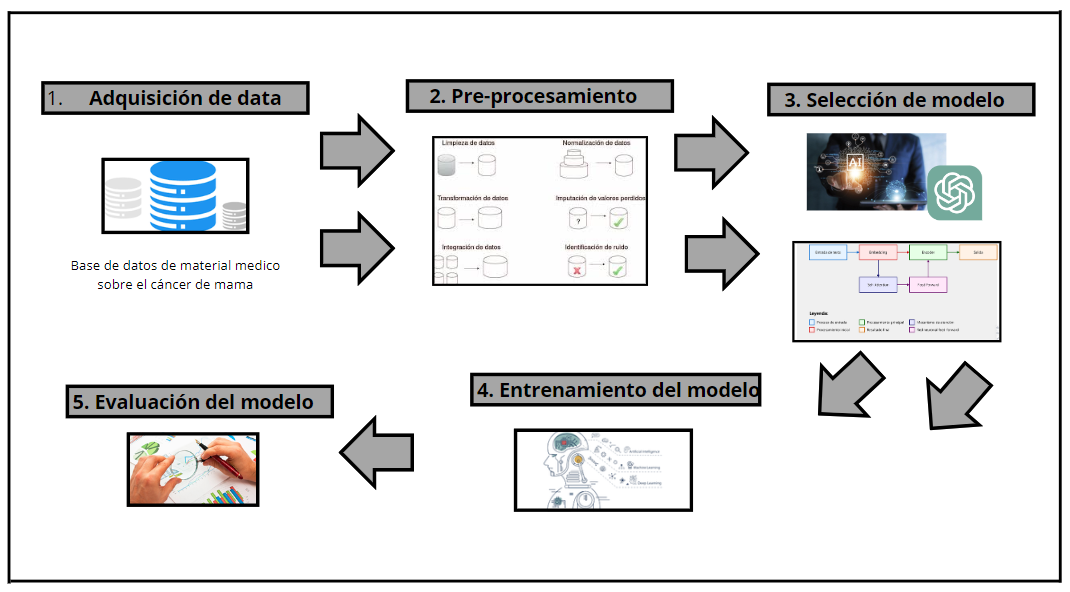
\includegraphics[width=\textwidth]{3/figures/MIsolucion.png}
	\caption{Metodología de la investigación}
	\label{14:fig}
\end{figure}
\begin{figure}[ht]
	\centering
	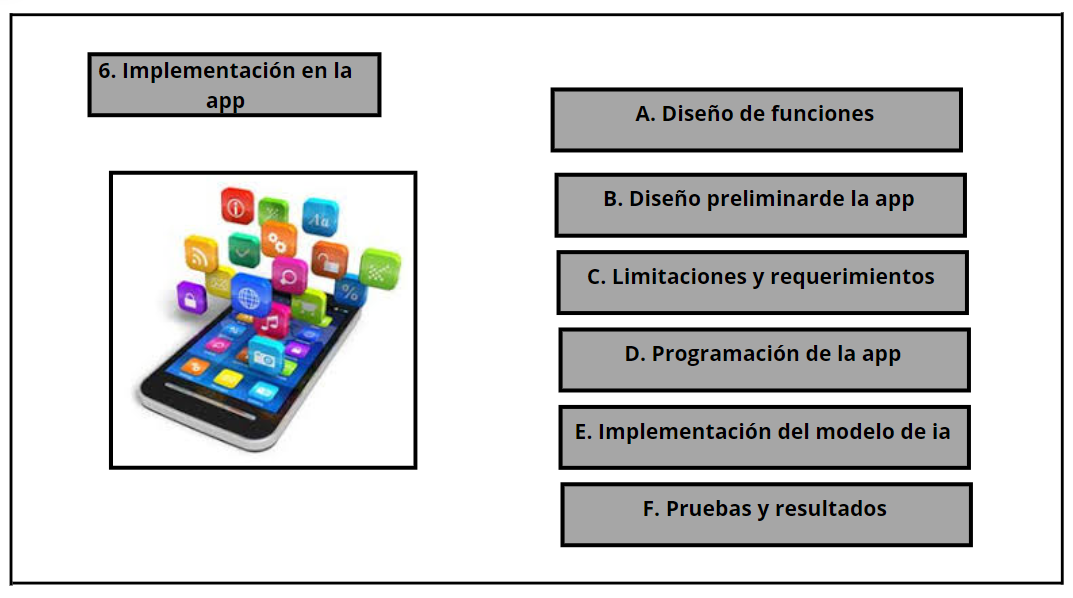
\includegraphics[width=\textwidth]{3/figures/MI2.png}
	\caption{Metodología de la investigación}
	\label{14:fig}
\end{figure}

\subsubsection{Adquisición de Datos}
La calidad de los datos es fundamental para entrenar un modelo de IA generativa efectivo. Este paso debe garantizar datos ricos, diversos y representativos del dominio médico y emocional.

\textbf{Fuentes de datos específicas:}
\begin{itemize}
    \item \textit{Bases de datos textuales médicas:} PubMed, MIMIC-III (datos clínicos anonimizados), OncoKB, guías clínicas internacionales como NCCN Guidelines y ESMO Guidelines.
    \item \textit{Transcripciones de interacciones médico-paciente:} Conversaciones reales o simuladas representativas de preguntas y respuestas comunes.
    \item \textit{Datos emocionales o psicológicos:} Encuestas sobre ansiedad y estrés en pacientes oncológicos, datos de plataformas de telemedicina y análisis de textos en foros.
\end{itemize}

\textbf{Proceso de recopilación:}
\begin{itemize}
    \item Colaboraciones con hospitales o clínicas para obtener datos anonimizados.
    \item Uso de bases públicas disponibles.
    \item \textit{Web scraping} en páginas confiables con permisos legales.
\end{itemize}

\textbf{Normativas éticas:}
\begin{itemize}
    \item Cumplir con estándares como GDPR o HIPAA para garantizar privacidad.
    \item Revisiones éticas continuas durante todo el proceso.
\end{itemize}

\subsection{Preprocesamiento de Datos}
El preprocesamiento asegura que los datos estén organizados y listos para ser utilizados por el modelo.

\textbf{Pasos principales:}
\begin{itemize}
    \item \textit{Limpieza del texto:} Eliminación de información irrelevante, corrección de errores tipográficos, y normalización de abreviaturas médicas.
    \item \textit{Tokenización:} Dividir los textos en palabras, subpalabras o frases según el enfoque del modelo.
    \item \textit{Etiquetado:} Clasificar información en categorías como diagnóstico, tratamiento, emociones y preguntas frecuentes.
    \item \textit{Normalización:} Convertir textos a minúsculas, eliminar caracteres especiales y estandarizar unidades médicas.
\end{itemize}

\textbf{Enriquecimiento de datos:}
\begin{itemize}
    \item Realizar \textit{data augmentation} textual para diversificar el dataset.
\end{itemize}


\subsection{Selección del Modelo}
Dado que el objetivo es implementar un modelo generativo eficiente, los Transformers son la elección más adecuada.

\textbf{Modelos a considerar:}
\begin{itemize}
    \item \textit{GPT (Generative Pre-trained Transformer):} Ideal para generar respuestas empáticas y médicamente correctas.
    \item \textit{T5 (Text-to-Text Transfer Transformer):} Versátil para tareas de entrada y salida de texto.
    \item \textit{BERT:} Orientado a la comprensión textual, útil como complemento para análisis de estados emocionales.
    \item \textit{Vision Transformers (ViT):} Opcional si se incluyen imágenes médicas.
\end{itemize}


\subsubsection{Motivación}
\begin{itemize}
    \item Los Transformers tienen capacidades avanzadas para manejar texto contextual y tareas personalizadas.
\end{itemize}

\subsection{Entrenamiento del Modelo}
El entrenamiento es la etapa más crítica y se divide en varias subfases.

\textbf{Preparación del entrenamiento:}
\begin{itemize}
    \item \textit{División del dataset:}
    \begin{itemize}
        \item \textbf{70-80\% entrenamiento:} Ajuste de pesos del modelo.
        \item \textbf{10-15\% validación:} Optimización de hiperparámetros y evaluación durante el proceso.
        \item \textbf{10-15\% pruebas:} Evaluación de precisión final.
    \end{itemize}
    \item \textit{Hiperparámetros clave:}
    \begin{itemize}
        \item Tamaño del \textit{batch:} 16-64 (dependiendo de la GPU).
        \item Tasa de aprendizaje: 1e-4 o 1e-5 para modelos preentrenados.
        \item Número de \textit{epochs:} 20-50 según el tamaño del dataset.
    \end{itemize}
\end{itemize}

\textbf{Técnicas de entrenamiento:}
\begin{itemize}
    \item \textit{Fine-tuning:} Adaptación de modelos preentrenados al dominio específico.
    \item \textit{Entrenamiento desde cero:} Útil si se requieren características únicas no presentes en modelos existentes.
    \item \textit{Regularización:} Uso de técnicas como Dropout para evitar sobreajuste.
\end{itemize}

\subsection{Evaluación del Modelo}
La evaluación asegura que el modelo funcione correctamente y sea útil para los pacientes y médicos.

\textbf{Métricas de desempeño:}
\begin{itemize}
    \item \textit{Perplejidad:} Evalúa la capacidad del modelo para predecir palabras.
    \item \textit{BLEU/ROUGE:} Miden la similitud entre el texto generado y de referencia.
    \item \textit{Validación con expertos:} Médicos revisan las respuestas generadas.
    \item \textit{Pruebas A/B:} Comparación con métodos tradicionales.
\end{itemize}

\section{Cronograma de actividades y presupuesto (Hasta la fecha actual}
\subsection{Cronograma de actividades}
\begin{figure}[ht]
	\centering
	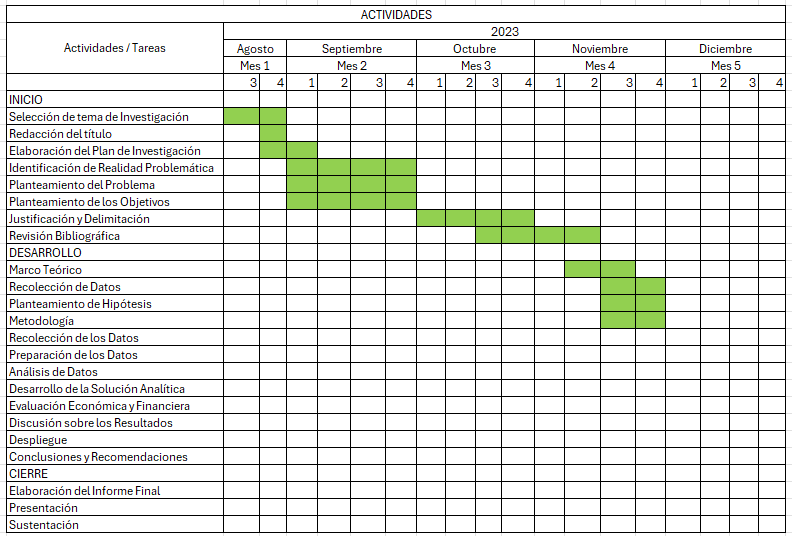
\includegraphics[width=\textwidth]{3/figures/Cronograma de actividades hasta la fecha.png}
	\caption{Cronograma de actividades}
	\label{15:fig}
\end{figure}

\subsection{Presupuesto}
\begin{figure}[ht]
	\centering
	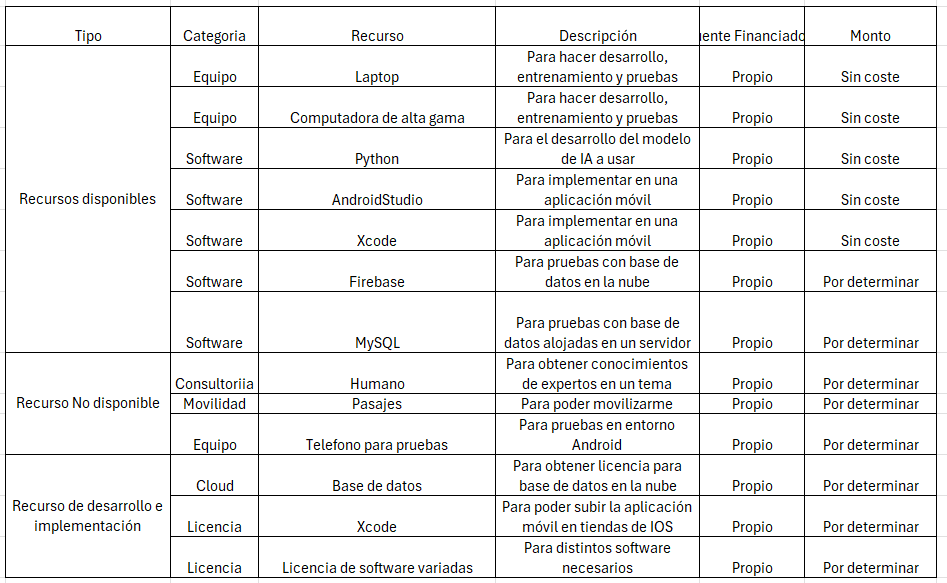
\includegraphics[width=\textwidth]{3/figures/Recursos.png}
	\caption{Recursos necesarios}
	\label{16:fig}
\end{figure}

\chapter{DESARROLLO DEL EXPERIMENTO}
\section{X}

Hello, here is some text without a meaning.  This text should 
show what a printed text will look like at this place.  If you 
read this text, you will get no information.  Really?  Is there 
no information?  Is there a difference between this text and some 
nonsense like ``Huardest gefburn?  Kjift " not at all!...

\begin{table}
	\centering
	\begin{tabular}{l|r}
		Item & Quantity \\\hline
		Widgets & 42 \\
		Gadgets & 13
	\end{tabular}
	\caption{\label{tab:widgets1}An example table.}
\end{table}

\section{Y}

 Nisi porta lorem mollis aliquam ut porttitor leo. Aenean pharetra magna ac placerat vestibulum. Est placerat in egestas erat imperdiet sed euismod. Velit euismod in pellentesque massa placerat. Enim praesent elementum facilisis leo vel fringilla. Ante in nibh mauris cursus mattis molestie a iaculis. Erat pellentesque adipiscing commodo elit at imperdiet dui accumsan sit. Porttitor lacus luctus accumsan tortor posuere ac ut. Tortor at auctor urna nunc id. A iaculis at erat pellentesque adipiscing commodo elit. 


\section{Z}

Nisi porta lorem mollis aliquam ut porttitor leo. Aenean pharetra magna ac placerat vestibulum. Est placerat in egestas erat imperdiet sed euismod. Velit euismod in pellentesque massa placerat. Enim praesent elementum facilisis leo vel fringilla. Ante in nibh mauris cursus mattis molestie a iaculis. Erat pellentesque adipiscing commodo elit at imperdiet dui accumsan sit. Porttitor lacus luctus accumsan tortor posuere ac ut. Tortor at auctor urna nunc id. A iaculis at erat pellentesque adipiscing commodo elit. 

El paper es citado  y el otro paper .

\chapter{ANÁLISIS Y DISCUSIÓN DE RESULTADOS}
\section{X}

Hello, here is some text without a meaning.  This text should 
show what a printed text will look like at this place.  If you 
read this text, you will get no information.  Really?  Is there 
no information?  Is there a difference between this text and some 
nonsense like ``Huardest gefburn?  Kjift " not at all!...

\begin{table}
	\centering
	\begin{tabular}{l|r}
		Item & Quantity \\\hline
		Widgets & 42 \\
		Gadgets & 13
	\end{tabular}
	\caption{\label{tab:widgetxcxs}An example table.}
\end{table}

\section{Y}

Nisi porta lorem mollis aliquam ut porttitor leo. Aenean pharetra magna ac placerat vestibulum. Est placerat in egestas erat imperdiet sed euismod. Velit euismod in pellentesque massa placerat. Enim praesent elementum facilisis leo vel fringilla. Ante in nibh mauris cursus mattis molestie a iaculis. Erat pellentesque adipiscing commodo elit at imperdiet dui accumsan sit. Porttitor lacus luctus accumsan tortor posuere ac ut. Tortor at auctor urna nunc id. A iaculis at erat pellentesque adipiscing commodo elit. 


\section{Z}

Nisi porta lorem mollis aliquam ut porttitor leo. Aenean pharetra magna ac placerat vestibulum. Est placerat in egestas erat imperdiet sed euismod. Velit euismod in pellentesque massa placerat. Enim praesent elementum facilisis leo vel fringilla. Ante in nibh mauris cursus mattis molestie a iaculis. Erat pellentesque adipiscing commodo elit at imperdiet dui accumsan sit. Porttitor lacus luctus accumsan tortor posuere ac ut. Tortor at auctor urna nunc id. A iaculis at erat pellentesque adipiscing commodo elit.

\chapter{CONCLUSIONES Y RECOMENDACIONES}
\section{Conclusiones}

Hello, here is some text without a meaning.  This text should 
show what a printed text will look like at this place.  If you 
read this text, you will get no information.  Really?  Is there 
no information?  Is there a difference between this text and some 
nonsense like ``Huardest gefburn?  Kjift " not at all!...



\section{Recomendaciones}

Nisi porta lorem mollis aliquam ut porttitor leo. Aenean pharetra magna ac placerat vestibulum. Est placerat in egestas erat imperdiet sed euismod. Velit euismod in pellentesque massa placerat. Enim praesent elementum facilisis leo vel fringilla. Ante in nibh mauris cursus mattis molestie a iaculis. Erat pellentesque adipiscing commodo elit at imperdiet dui accumsan sit. Porttitor lacus luctus accumsan tortor posuere ac ut. Tortor at auctor urna nunc id. A iaculis at erat pellentesque adipiscing commodo elit. 



%%Anexos
\appendix
\renewcommand{\appendixname}{Anexos}
\renewcommand{\appendixtocname}{Anexos}
\renewcommand{\appendixpagename}{Anexos}
\clearpage
\addappheadtotoc
\appendixpage
\chapter{Anexo I: Matriz de Consistencia}

\begin{table}[htbp]
\centering
\small
\begin{tabular}{|p{5cm}|p{5cm}|p{5cm}|}
\hline
\textbf{Problema} & \textbf{Objetivos} & \textbf{Hipótesis} \\
\hline
¿De qué manera una aplicación móvil mediante el uso de inteligencia artificial generativa puede contribuir al control, monitoreo integral y educación de los pacientes con cáncer de mama? 
& Desarrollar una aplicación móvil basada en Inteligencia Artificial generativa para el monitoreo integral y el control de pacientes con cáncer, que mejore la adherencia al tratamiento, el seguimiento de signos vitales, el soporte emocional y conocimiento sobre la enfermedad. 
& El desarrollo de una aplicación móvil que emplea Inteligencia Artificial generativa mejorará significativamente el monitoreo integral, el control y la educación de los pacientes con cáncer de mama. \\
\hline
\end{tabular}
\caption{Desarrollo de una aplicación móvil: Problema Principal, Objetivo y Hipótesis}
\label{tabla_principal}
\end{table}

\begin{table}[htbp]
\centering
\small
\begin{tabular}{|p{5cm}|p{5cm}|p{5cm}|}
\hline
\textbf{Problema específico} & \textbf{Objetivo específico} & \textbf{Hipótesis específica} \\
\hline
¿Qué base de datos se deben usar para entrenar el modelo de IA para ofrecer respuestas óptimas? 
& Identificar las bases de datos especializadas que se pueden integrar para entrenar el modelo de IA generativa de la aplicación móvil. 
& La implementación de un modelo de IA generativa entrenado con bases de datos médicas especializadas en el cáncer de mama permitirá a la aplicación móvil proporcionar respuestas precisas y personalizadas a las consultas de los pacientes, mejorando su comprensión de la enfermedad y el tratamiento. \\
\hline
¿De qué manera una aplicación móvil puede proporcionar soporte emocional a los pacientes oncológicos? 
& Implementar un sistema de IA generativa que proporcione soporte emocional personalizado en función del estado anímico del paciente. 
& La implementación de un sistema de soporte emocional automatizado mejorará el bienestar emocional de los pacientes, reduciendo su ansiedad y mejorando su calidad de vida. \\
\hline
¿Qué funcionalidades de una aplicación móvil son esenciales para el monitoreo de signos vitales en pacientes con cáncer? 
& Desarrollar un sistema de monitoreo de signos vitales en tiempo real que notifique a los pacientes sobre anomalías. 
& La integración de un sistema de monitoreo de signos vitales basado en IA reducirá las complicaciones relacionadas con la falta de detección temprana de problemas. \\
\hline
¿Cómo puede una aplicación móvil proporcionar información personalizada y actualizada sobre el cáncer de mama utilizando IA generativa? 
& Desarrollar una funcionalidad que permita a los pacientes recibir información personalizada y actualizada sobre su condición. 
& La implementación de un sistema que proporcione información personalizada mejorará el conocimiento del paciente sobre su enfermedad y su tratamiento. \\
\hline
¿Qué modelo de IA generativa se va a implementar para que las funciones de la aplicación móvil funcionen correctamente? 
& Seleccionar y optimizar el modelo de IA generativa más adecuado para integrar todas las funciones de la aplicación móvil de manera eficiente. 
& La implementación de un modelo de IA generativa optimizado permitirá que todas las funciones de la aplicación móvil (soporte emocional, monitoreo de signos vitales, información personalizada) funcionen de manera eficiente y precisa. \\
\hline
\end{tabular}
\caption{Desarrollo de una aplicación móvil: Problemas Específicos, Objetivos y Hipótesis}
\label{tabla_especificos}
\end{table}

\chapter{Anexo II: Árbol de problemas y de objetivos}

\begin{figure}[ht]
	\centering
	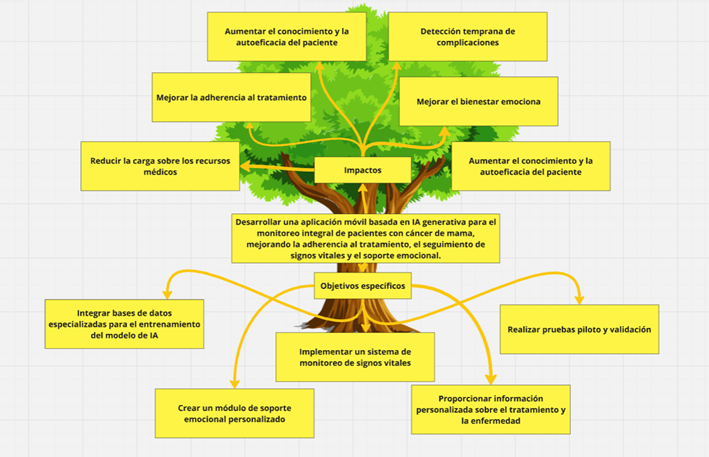
\includegraphics[width=1.1\textwidth]{anexos/Imagen1.png}
	\caption{Árbol de problemas}
	\label{8:fig}
\end{figure}

\begin{figure}[ht]
	\centering
	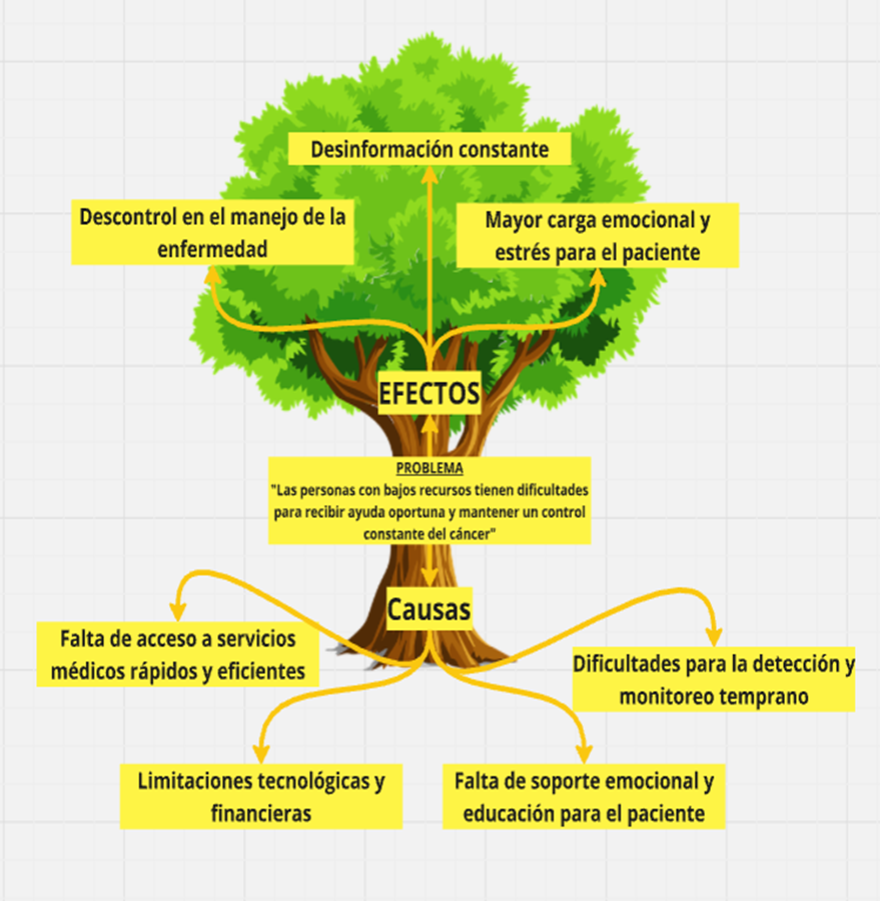
\includegraphics[width=1.1\textwidth]{anexos/Imagen2.png}
	\caption{Árbol de objetivos}
	\label{8:fig}
\end{figure}


% %%Bibliografia
%\bibliographystyle{apalike} % Title is link if provided
%\renewcommand{\bibname}{BIBLIOGRAFÍA} % changes the header; default: Bibliography
\nocite{*}
\printbibliography[heading=bibintoc,title={BIBLIOGRAFÍA}]
%\bibliography{biblio/references} % adjust this to fit your BibTex file
\end{document}